
\documentclass{article}
\usepackage{hyperref}
\usepackage{enumitem}
\usepackage{graphicx}
\usepackage{amsmath}
\usepackage{mathpazo}
\usepackage{xcolor}
\usepackage{float}
\usepackage{listings}

\definecolor{pblue}{rgb}{0.13,0.13,1}
\definecolor{pgreen}{rgb}{0,0.5,0}
\definecolor{pred}{rgb}{0.9,0,0}
\definecolor{pgrey}{rgb}{0.46,0.45,0.48}
\definecolor{backcolour}{rgb}{0.95,0.95,0.92}

\lstdefinestyle{style_compact}{
    language=Java,
    backgroundcolor=\color{backcolour},         % keep same background
    commentstyle=\color{pgreen},                % reuse your colors
    keywordstyle=\color{pblue},
    stringstyle=\color{pred},
    numberstyle=\scriptsize\color{pgrey},       % smaller line‐number font
    basicstyle=\ttfamily\scriptsize,            % very small code font
    columns=fullflexible,                       % no extra space for monospaced
    keepspaces=true,
    breaklines=true,
    breakatwhitespace=true,
    showspaces=false,
    showstringspaces=false,
    showtabs=false,
    tabsize=2,
    numbers=left,
    stepnumber=1,
    numbersep=3pt,                              % tighter gap to numbers
    xleftmargin=8pt,                            % slight indent
    xrightmargin=8pt,
    aboveskip=2pt,                              % minimal vertical space
    belowskip=2pt,
    lineskip=-0.5pt,                            % pull lines closer
    frame=single,                               % optional frame
}
\lstset{style=style_compact}

\usepackage[export]{adjustbox}
\usepackage{multicol}
\usepackage{caption}
\usepackage[a4paper,
            bindingoffset=0.2in,
            left=0.5in,
            right=0.5in,
            top=0.5in,
            bottom=0.5in,
            footskip=.25in]{geometry}


\begin{document}
\title{MS Technical Paper: \\ Placement Algorithms for Heterogeneous FPGAs}
\author{Brian B Cheng \\ Rutgers University Department of Electrical and Computer Engineering}


\date{}
\maketitle


\begin{multicols}{2}

\section{Keywords}
\begin{itemize}
\item FPGA, EDA, Placement, Simulated Annealing, Optimization, RapidWright
\end{itemize}

\section{Abstract}
Placement remains one of the most computationally demanding stages of FPGA computer-aided design (CAD) flows, directly influencing routability, timing, and design productivity. 
This paper presents a modular placement framework targeting Xilinx 7-Series devices, implemented using the RapidWright API. 
The flow first clusters multi-cell structures (such as CARRY4 chains, DSP48E1 cascades, and LUT–FF pairs) into prepacked groups, then maps them to physical sites before applying a simulated annealing (SA) placer. 
The SA engine minimizes half-perimeter wirelength (HPWL) using a geometric cooling schedule, with support for both random and directed moves. 
The result is a legal, wirelength-optimized placement that forms a foundation for experimenting with alternative cost functions and analytical or hybrid placement strategies.


\section{Introduction}

Field-Programmable Gate Arrays (FPGAs) have witnessed rapid growth in capacity and versatility, driving significant advances in computer-aided design (CAD) and electronic design automation (EDA) methodologies. 
Since the early-to-mid 2000s, the stagnation of single-processor performance relative to the rapid increase in integrated circuit sizes has led to a design productivity gap, where the computational effort for designing complex chips continues to rise. 
FPGA CAD flows mainly encompass synthesis, placement, and routing; all of which are NP-hard problems, of which placement is one of the most time-consuming processes. 
Inefficient placement strategy not only extends design times from hours to days, thereby elevating cost and reducing engineering productivity, but also limits the broader adoption of FPGAs by software engineers who expect compile times akin to those of software compilers like {\tt gcc}. 

For these reasons, FPGA placement remains a critical research effort even today. 
In this paper, we study and implement established placement methods. 
To do this, we use the RapidWright API, which is a semi-open-source research effort from AMD/Xilinx that enables custom solutions to FPGA design implementations and design tools that are not offered by their industry-standard FPGA environment, Vivado. 
We implement multiple variations of simulated annealing placers for Xilinx's 7-series FPGAs, with an emphasis on minimizing total wirelength while mitigating runtime. 
Our implementation is organized into three consecutive substages. 
The \textbf{prepacking} stage involves traversing a raw EDIF netlist to identify recurring cell patterns—such as CARRY chains, DSP cascades, and LUT-FF pairs—that are critical for efficient mapping and legalization. 
In the subsequent \textbf{packing} stage, these identified patterns, along with any remaining loose cells, are consolidated into \texttt{SiteInst} objects that encapsulate the FPGA’s discrete resource constraints and architectural nuances. 
Finally, the \textbf{placement} stage employs a simulated annealing (SA) algorithm to optimally assign \texttt{SiteInst} objects to physical \texttt{Sites}, aiming to minimize total wirelength while the constraints of the 7-series architecture. 

Simulated annealing iteratively swaps placement objects guided by a cost function that decides which swaps should be accepted or rejected. 
Hill climbing is permitted by occasionally accepting moves that increase cost, in hope that such swaps may later lead to a better final solution. 
SA remains a popular approach in FPGA placement research due to its simplicity and robustness in handling the discrete architectural constraints of FPGA devices. 
While SA yields surprisingly good results given relatively simple rules, it is ultimately a heuristic approach that explores the vast placement space by making random moves. 
Most of these moves will be rejected, meaning that SA must run many iterations, usually hundreds to thousands, to arrive at a desirable solution. 

In the ASIC domain, where placers must handle designs with millions of cells, the SA approach has largely been abandoned in favor of analytical techniques, owing to SA's runtime and poor scalability. 
Modern FPGA placers have also followed suit, as new legalization strategies allow FPGA placers to leverage traditionally ASIC placement algorithms and adapt them to the discrete constraints of FPGA architectures. 
While this paper does not present a working analytical placer, it will explore ways to build upon our existing infrastructure (prepacker and packer) to replace SA with AP. 

The paper first begins by elaborating on general FPGA architecture and then specifically the Xilinx 7-Series architecture. 
Then, the paper will elaborate on the FPGA design flow, then the role that the RapidWright API plays in the design flow. 
We explain in detail each of these concepts for a broader audience as they provide much needed context for FPGA placement algorithms as a concept. 
However, readers who are already familiar with these concepts can skip directly to the RapidWright API section \ref{sec:rapidwright_api} or to the Simulated Annealing section \ref{sec:simulated_annealing}. 

\section{FPGA Architecture History}
Before any work can begin on an FPGA placer, it is necessary to understand both the objects being placed and the medium in which they are placed.
Configurable logic devices have undergone significant evolution over the past four decades. 
We will briefly review the evolution of configurable logic architecture starting in the 1970s and quickly work our way up to modern day FPGA architecture. 

\textbf{PLA:} \quad
The journey began with the Programmable Logic Array (PLA) in the early 1970s. 
The PLA implemented output logic using a programmable-OR and programmable-AND plane that formed a sum-of-products equation for each output through programmable fuses. 
Around the same time, the Programmable Array Logic (PAL) was introduced. 
The PAL simplified the PLA by fixing the OR gates, resulting in a fixed-OR, programmable-AND design, which sacrificed some logic flexibility to simplify its manufacture. 
Figure \ref{fig:pal_2} shows one such PAL architecture. 

\textbf{CPLD:} \quad 
Later in the same decade came the Complex Programmable Logic Device (CPLD), which took the form of an array of Configurable Logic Blocks (CLBs). 
These CLBs were typically modified PAL blocks that included the PAL itself along with macrocells such as flip-flops, multiplexers, and tri-state buffers. 
The CPLD functioned as an array of PALs connected by a central programmable switch matrix and could be programmed using a hardware description language (HDL) like VHDL. 
Figure \ref{fig:cpld} shows one such CPLD architecture. 
\\

{
    \centering
    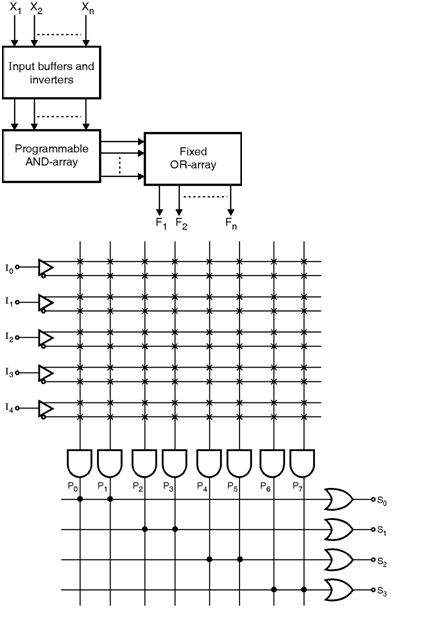
\includegraphics[width=\columnwidth]{figures/pal_2.png}
    \captionof{figure}{PAL architecture with 5 inputs, 8 programmable AND gates and 4 fixed OR gates}
    \label{fig:pal_2}
    % https://www.electronics-tutorial.net/Programmable-Logic-Device-Architectures/Programmable-Logic-Devices/Programmable-Array-Logic-PAL/
    % https://www.naukri.com/code360/library/difference-between-pla-and-pal 
}

\newcolumn

\textbf{Homogeneous FPGA:} \quad 
The mid-1980s saw the introduction of homogeneous FPGAs, which were built as a grid of CLBs. 
Rather than using a central programmable switch matrix as in CPLDs, FPGAs adopted an island style architecture in which each CLB is surrounded on all sides by programmable routing resources, as shown in Figure \ref{fig:fpga}. 
The first commercially viable FPGA, produced by Xilinx in 1984, featured 16 CLBs arranged in a 4x4 grid. 
As FPGA technology advanced, CLBs were redesigned to use lookup tables (LUTs) instead of PAL arrays for greater logic density. 
The capacity of an FPGA was often measured by how many logical elements or CLBs it offered, which grew from hundreds to thousands and now to hundreds of thousands of CLBs.
\\ 

{
    \centering
    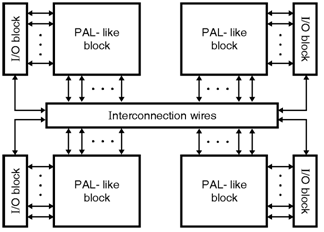
\includegraphics[width=0.8\columnwidth]{figures/cpld.png}
    \captionof{figure}{CPLD architecture with 4 CLBs (PAL-like blocks)}
    \label{fig:cpld}
    % https://www.electronics-tutorial.net/Programmable-Logic-Device-Architectures/CPLD/Complex-Programmable-Logic-Device-CPLDs/
}
{
    \centering
    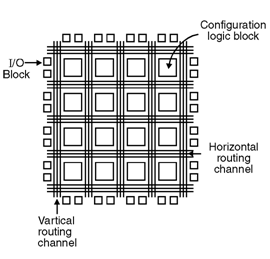
\includegraphics[width=\columnwidth]{figures/homogenous_fpga.png}
    \captionof{figure}{A homogeneous island-style FPGA architecture with 16 CLBs in a grid.}
    \label{fig:fpga}
    % https://www.electronics-tutorial.net/Programmable-Logic-Device-Architectures/FPGA/Field-programmable-gate-array-FPGA/
}

\newpage

{
    \centering
    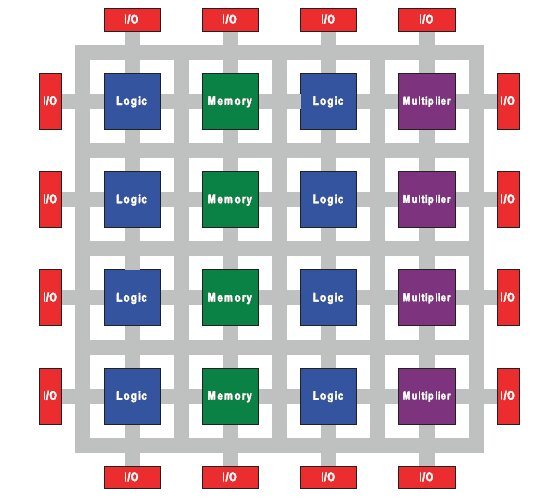
\includegraphics[width=\columnwidth]{figures/heterogenous_fpga_3.jpg}
    \captionof{figure}{A heterogeneous island-style FPGA with a mix of CLBs and macrocells.}
    \label{fig:fpga}
    % https://www.electronics-tutorial.net/Programmable-Logic-Device-Architectures/FPGA/Field-programmable-gate-array-FPGA/
}
\vspace{0.25cm}

\textbf{Heterogenous FPGA:} \quad 
This brings us to modern day FPGA architectures. 
To meet the needs of increasingly complex designs, FPGA vendors introduced heterogeneous FPGAs. 
In these devices, hard macros such as Block RAM (BRAM) and Digital Signal Processing (DSP) slices are integrated into the programmable logic fabric along with CLBs, like shown in Figure \ref{fig:fpga}. 
This design enables the direct instantiation of common subsystems like memories and multipliers, without having to recreate them from scratch using CLBs. 
Major vendors such as Xilinx (AMD) and Altera (Intel) now employ heterogeneous island-style architectures in their devices. 
As designs become increasingly large and complex, FPGAs meet the demand by becoming increasingly heterogenous, incorporating a wider variety of hard macros into the fabric. 



\section{Xilinx 7-Series Architecture}
\label{sec:7_series}
The Xilinx 7-Series devices, first introduced in 2010, follow a heterogeneous island-style architecture as discussed previously. 
Although the 7-Series was later superseded in 2013 by the UltraScale architecture, the 7-Series remains highly relevant due to its accessibility, wide availability, and compatibility with open-source tooling. 
Representative sub-families include Artix-7, Kintex-7, Virtex-7, and Zynq-7000, each designed with different performance and cost trade-offs but all follow the core 7-Series architecture.


Figure~\ref{fig:hierarchy_4} illustrates a high-level view of the hierarchical organization of a 7-Series FPGA. 
At its lowest level, the device consists of a large array of atomic components called \emph{Basic Elements of Logic}~(\textbf{BELs}). 
These BELs encompass look-up tables (\textbf{LUTs}), flip-flops (\textbf{FFs}), block RAMs (\textbf{BRAMs}), DSP slices (\textbf{DSPs}), and the configurable interconnect fabric. 
They constitute the fundamental building blocks for implementing digital circuits on the FPGA.
Note how the Tile arrangement is columnar, where each column will have only one Tile type. 

To manage this complexity, Xilinx organizes these BELs into incrementally abstract structures. 
First, \textbf{BELs} are grouped into \textbf{Sites}. 
Each Site is embedded into a \textbf{Tile}, and Tiles are further arranged into \textbf{Clock Regions}. 
In some high-density devices, multiple Clock Regions may be consolidated into one or more \textbf{Super Logic Regions}~(SLRs). 
However, for the scope of this paper, we focus on Xilinx 7-Series devices with only a single SLR.

\end{multicols}
{
    \centering
    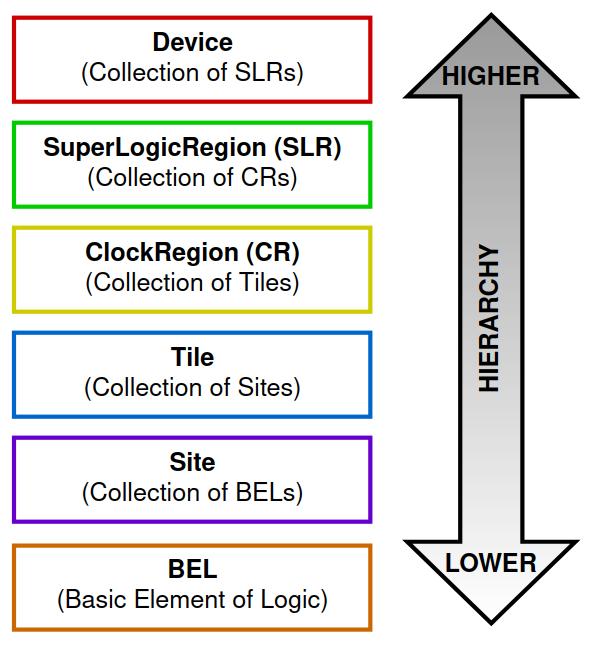
\includegraphics[valign=c, width=0.3\columnwidth]{figures/hierarchy_5.png}
    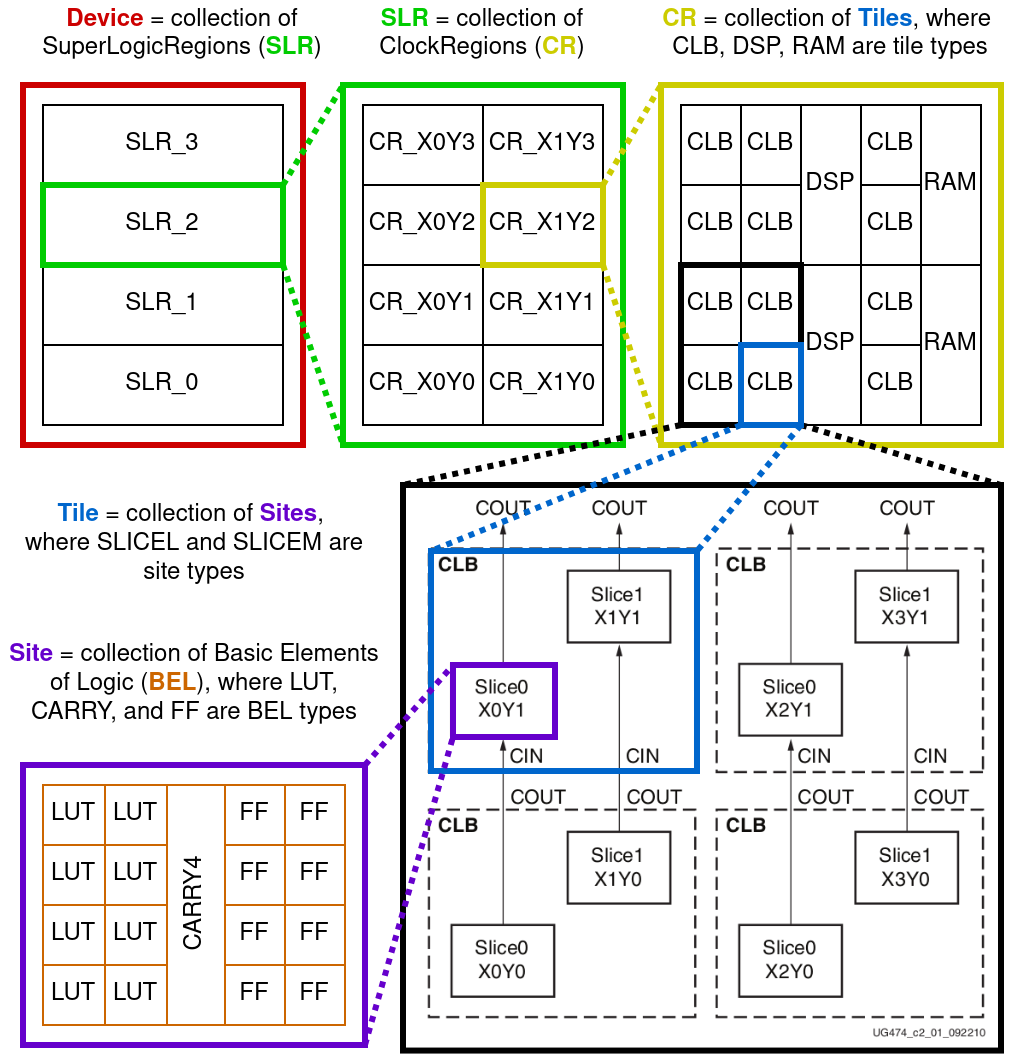
\includegraphics[valign=c, width=0.6\columnwidth]{figures/hierarchy_4.png}
    \captionof{figure}{Architecture Hierarchy of a Xilinx FPGA}
    \label{fig:hierarchy_4}
}
\vfill
\begin{multicols}{2}

\newpage
\subsection{CLB SLICEs}

In the 7-Series architecture, the term \emph{CLB} (Configurable Logic Block) refers to a \emph{CLB Tile} that contains two \emph{SLICE} Sites. 
Xilinx offers two variants of SLICE Sites: \textbf{SLICEL} and \textbf{SLICEM}.
\begin{itemize}
\item Each \texttt{SLICEL} has a set of BELs including eight \texttt{LUT}s, eight \texttt{FF}s, and one \texttt{CARRY4} adder. The \texttt{LUT} BELs in a \texttt{SLICEL} can only host \texttt{LUT} Cells. 
\item The \texttt{SLICEM} includes all the features of a \texttt{SLICEL} but its \texttt{LUT} BELs can host both \texttt{LUT} Cells, which are asynchronous ROM elements, or \texttt{RAM32M} Cells, which are synchronous 32-deep RAM elements. These cells are also referred to as \emph{Distributed RAM} in the Xilinx documentation.
    These cells can offer an alternative to the larger, more dedicated 18K-36K \texttt{RAMB18E1} cells when RAM resources are highly utilized. 
\end{itemize}
In a typical 7-Series device, approximately 75\% of the SLICE Sites are \texttt{SLICEL}s and 25\% are \texttt{SLICEM}s. 
A single CLB Tile can therefore host either two \texttt{SLICEL}s or one \texttt{SLICEL} and one \texttt{SLICEM}.
To simplify the problem space, however, we will only consider \texttt{SLICEL}s for general logic and use the dedicated \texttt{RAMB18E1} cells to implement RAM elements. 

The BELs in these SLICEs facilitate the bulk of the general programmability of the FPGA fabric. 
We will explain in detail the function and motivation behind these BELs. 


\textbf{LUTs} \quad
Combinational logic is universal to all HDL designs. 
As the their name suggests, a Look‑Up Table (LUT) map an input value to an output value. 
LUTs facilitate combinational logic by acting as tiny asynchronously‑accessed ROMs whose contents are fixed when the FPGA is programmed.  
For any boolean function, the synthesizer precalculates the boolean output to every possible input combination and stores the resulting truth table into a LUT's static memory. 
The inputs are then essentially treated as an address space that maps to a data value space in an asynchronous ROM. 
No explicit logic gates like NAND or XNOR are synthesized, contrary to what newcomers might expect from a "Field Programmable Gate Array". 

{
    \centering
    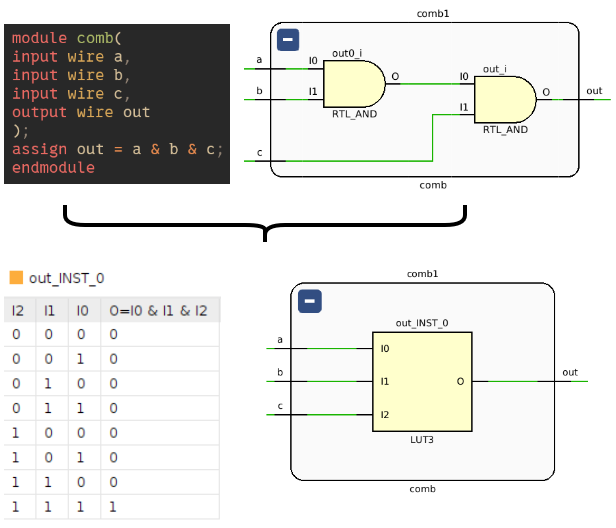
\includegraphics[width=\columnwidth]{figures/lut_synthesis.png}
    \captionof{figure}{LUT synthesis from user design}
    \label{fig:lut_synthesis}
}
\vspace{1.0cm}

In the 7‑Series devices, one LUT can facilitate any 6-input boolean function, or two 5-input functions, as long as they share the same input signals.  
The LUT can also host two independent boolean functions of up to 3 inputs each, even when the inputs are not shared.  
Functions requiring more than six unique inputs are decomposed across multiple cascaded LUTs.
Figure \ref{fig:lut_synthesis} shows an example of where a LUT is typically synthesized in a design entry. 


\textbf{FFs} \quad
FFs are synthesized to facilitate synchronous event-driven signal assignment. 
For most Verilog users, this generally means signal assignments wrapped in \texttt{always @(posedge clk)} statements. 
Figure \ref{fig:ff_synthesis} shows an example of where a FF is typically synthesized. 
The cell primitive \textbf{FDRE} is a type of FF and belongs to a family of D Flip Flops (DFFs) with Clock Enable (\texttt{CE}). 
\begin{itemize}
\item \texttt{FDCE} - DFF with CE and Asynchronous Clear
\item \texttt{FDPE} - DFF with CE and Asynchronous Preset
\item \texttt{FDSE} - DFF with CE and Synchronous Set
\item \texttt{FDRE} - DFF with CE and Synchronous Reset
\end{itemize}
In a typical HDL design, the vast majority of FFs will be synthesized as FDREs with the occasional FDSE, as it is generally good practice to keep FPGA designs synchronous. 
A FF BEL may also host a LATCH Cell, however, since they are generally bad practice in FPGA design, we will not consider latches in this paper. 

{
    \centering
    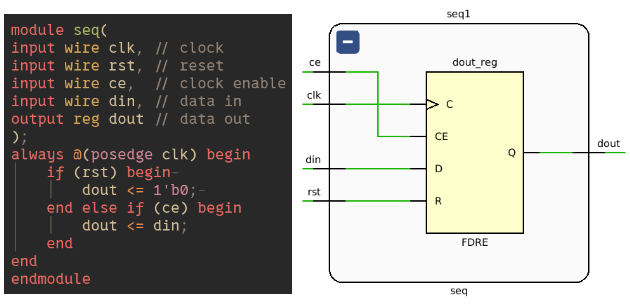
\includegraphics[width=\columnwidth]{figures/ff_synthesis.png}
    \captionof{figure}{FF synthesis from user design}
    \label{fig:ff_synthesis}
}
\vspace{1.0cm}

Up to eight (8) FFs can be placed within the same SLICE, but only if they all share a common Clock-Enable (CE) net and a common Set-Reset (SR) net.
This is because the SLICE has only one CE pin and one SR pin to interface with general routing. 
The CE and SR signals from these pins are broadcast intra-Site to all FFs within. 


\newpage
\textbf{LUT-FF Pairs} \quad
FPGA designs are very often modelled as a collection of Finite State Machines (FSM) like shown in Figure \ref{fig:fsm}.
Many times a design will also use pipelining, either to model signal buffers or shift registers, or to split up large combinational logic blocks into time slices to meet timing constraints. 
These common design structures result in many consecutive sections of combinational logic feeding into a vector of registers. 
The synthesizer naturally synthesizes these structures as consecutive pairs of LUTs feeding into FFs as shown in Figure \ref{fig:pipelining}. 
Figure \ref{fig:lut_ff_pair} shows an example of a synthesized LUT-FF Pair. 

Shown in Figure \ref{fig:intersite_intrasite} are two possible placements for a LUT-FF Pair on the physical device. 
On the right, the cells are placed across different Sites, thus the only way to route the net between the cells is through general inter-site routing. 
On the bottom left, the cells are placed within the same Site in the same lane, taking advantage of the intra-site routing without burdening the general router with additional inter-site routing. 
This is an important consideration to make while minimizing wirelength during placement. 


\vspace{1.0cm}
{
    \centering
    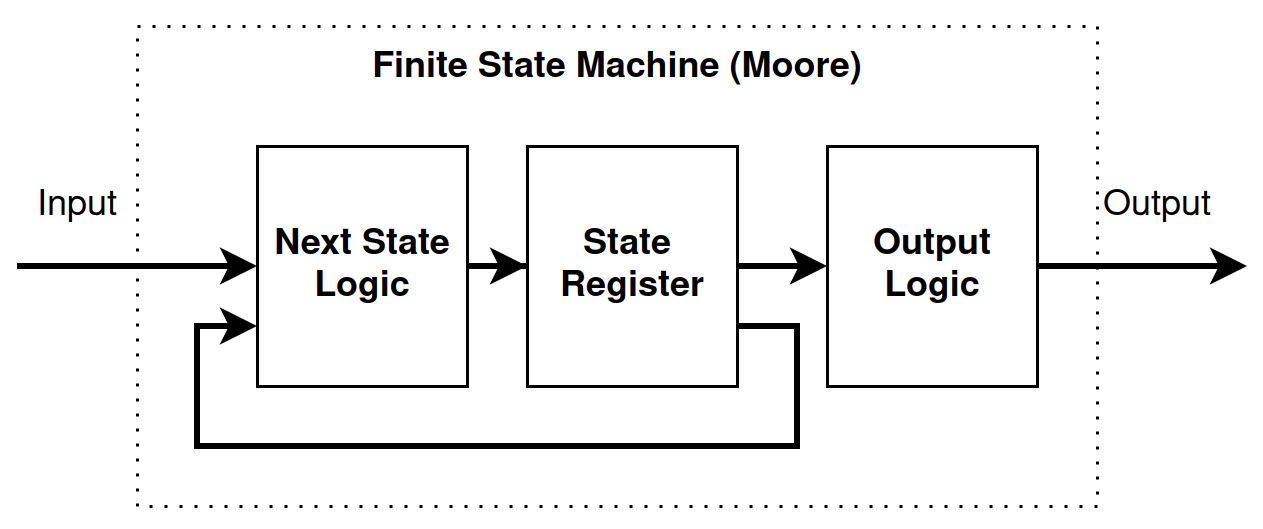
\includegraphics[width=\columnwidth]{figures/fsm.png}
    \captionof{figure}{Finite state machine (Moore)}
    \label{fig:fsm}
}
\vspace{1.0cm}

{
    \centering
    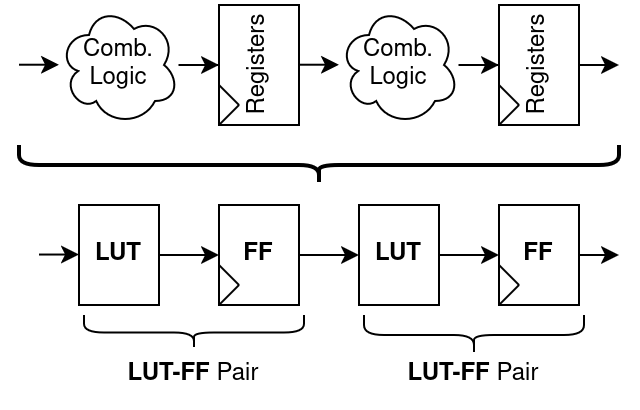
\includegraphics[width=0.9\columnwidth]{figures/pipelining.png}
    \captionof{figure}{Pipelining synthesized as consecutive LUT-FF pairs}
    \label{fig:pipelining}
}

\vfill
.
\newcolumn

{
    \centering
    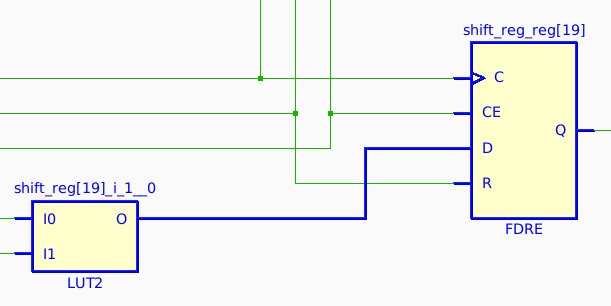
\includegraphics[width=0.9\columnwidth]{figures/lut_ff_pair.png}
    \captionof{figure}{A synthesized LUT-FF Pair}
    \label{fig:lut_ff_pair}
}
\vspace{1.0cm}

{
    \centering
    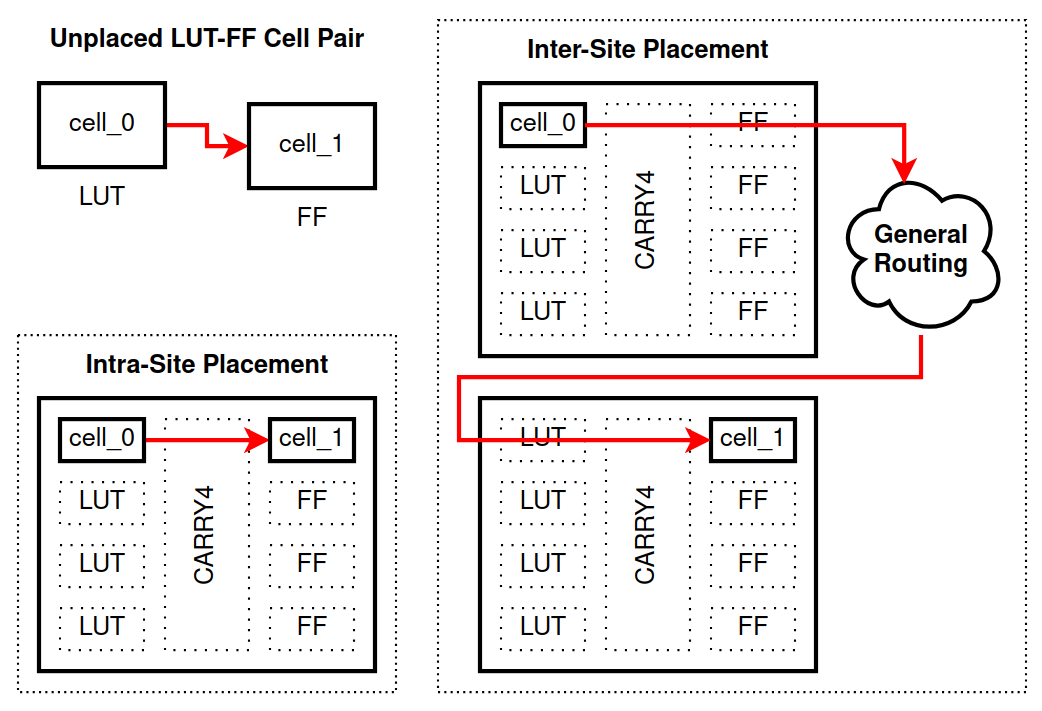
\includegraphics[width=\columnwidth]{figures/intersite_intrasite_2.png}
    \captionof{figure}{Intrasite vs Intersite LUT-FF Placement}
    \label{fig:intersite_intrasite}
}


\newpage
\textbf{CARRY} \quad
An FPGA design will also typically implement many adders, counters, subtractors, or comparators, all of which are based on binary addition. 
They are so ubiquitous that every that in the 7-Series architecture, every SLICE features a \texttt{CARRY4} BEL -- a 4-bit carry-lookahead (CLA) adder, a much better alternative to synthesizing adders via LUTs. 

\textbf{CARRY Chains} \quad
These \texttt{CARRY4} blocks can be chained across SLICEs to implement wide adders efficiently. 
The \texttt{CARRY4} BELs \emph{must} be chained vertically consecutively across SLICEs as the Carry-In (\texttt{CI}) and Carry-Out (\texttt{CO}) pins can only be routed this way. 
A \texttt{CARRY4} cell may also directly connect to LUTs and FFs, and should be placed in the same Site whenever possible to minimize wirelength. 
Shown in figure \ref{fig:carry_cell_group} shows how a \texttt{CARRY4} chain and associated LUTs and FFs can be placed across SLICEs. 


{
    \centering
    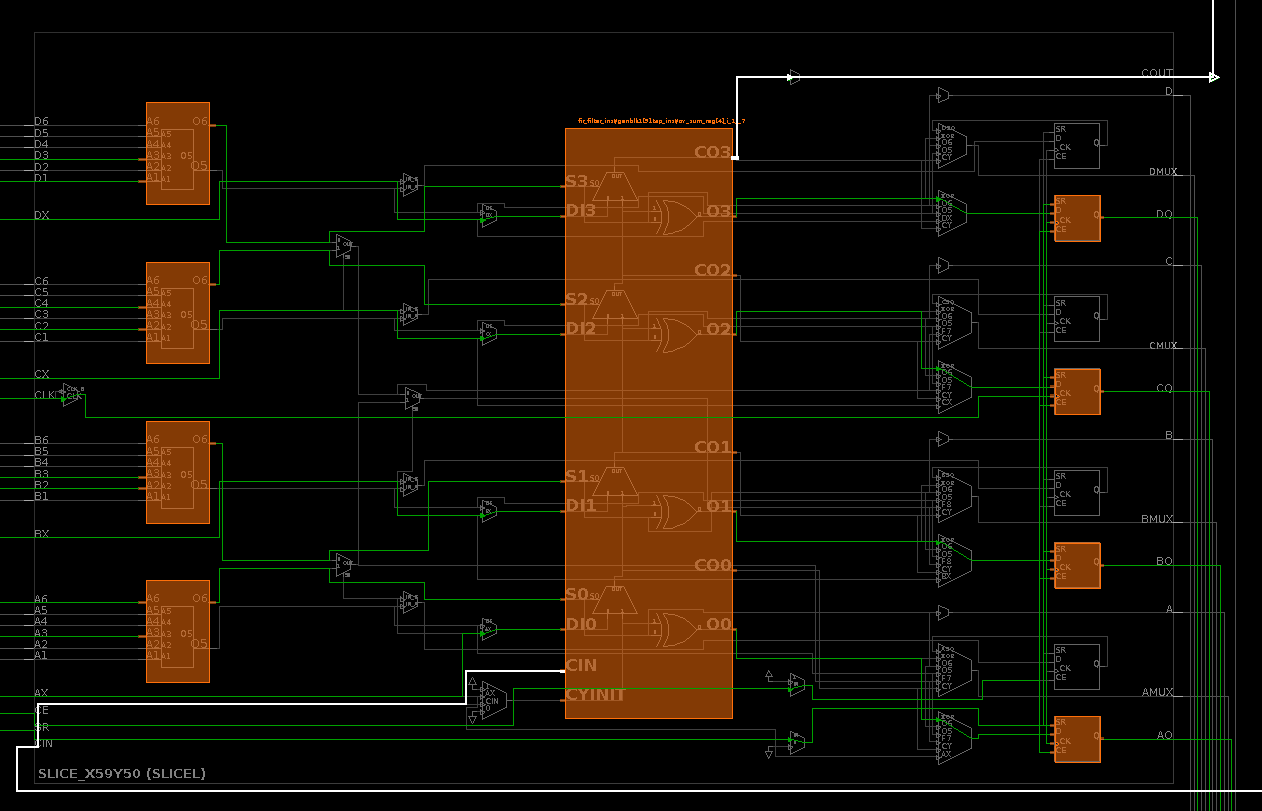
\includegraphics[width=\columnwidth]{figures/carry_cell_group.png}
    \captionof{figure}{A \texttt{SLICEL} with a \texttt{CARRY4} cell, 4 LUT cells, and 4 FF cells placed inside as shown in the Vivado device viewer}
    \label{fig:carry_cell_group}
}

{
    \centering
    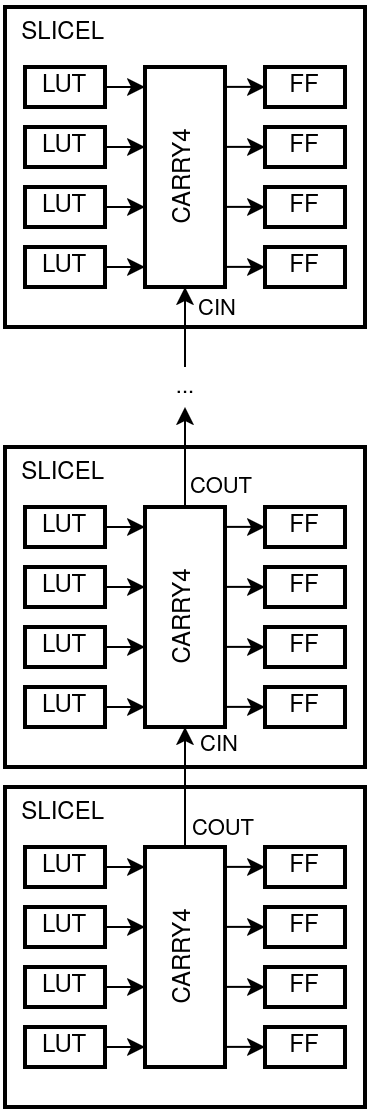
\includegraphics[valign=c, width=4.0cm]{figures/carry_chain_placement.png}
    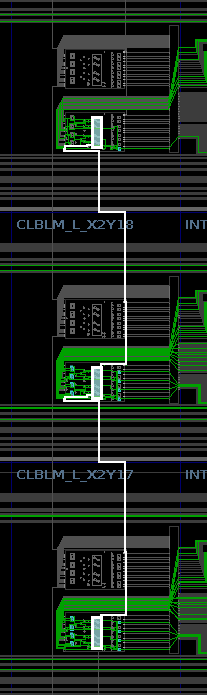
\includegraphics[valign=c, width=4.0cm]{figures/carry_chain_routes_3.png}
    \captionof{figure}{
        A \texttt{CARRY4} chain of size 3 placed across 3 SLICEs.
        \textbf{Left:} Simplified view, \textbf{Right:} As shown in the Vivado device viewer.
    }
    \label{fig:carry_cell_group}
}

\end{multicols}
% \vfill
{
    \centering
    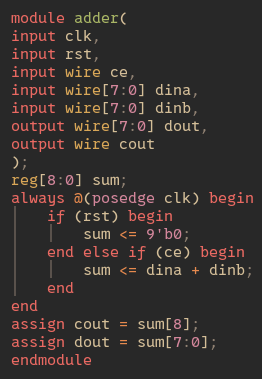
\includegraphics[valign=c, width=3.0cm]{figures/adder_synthesis.png}
    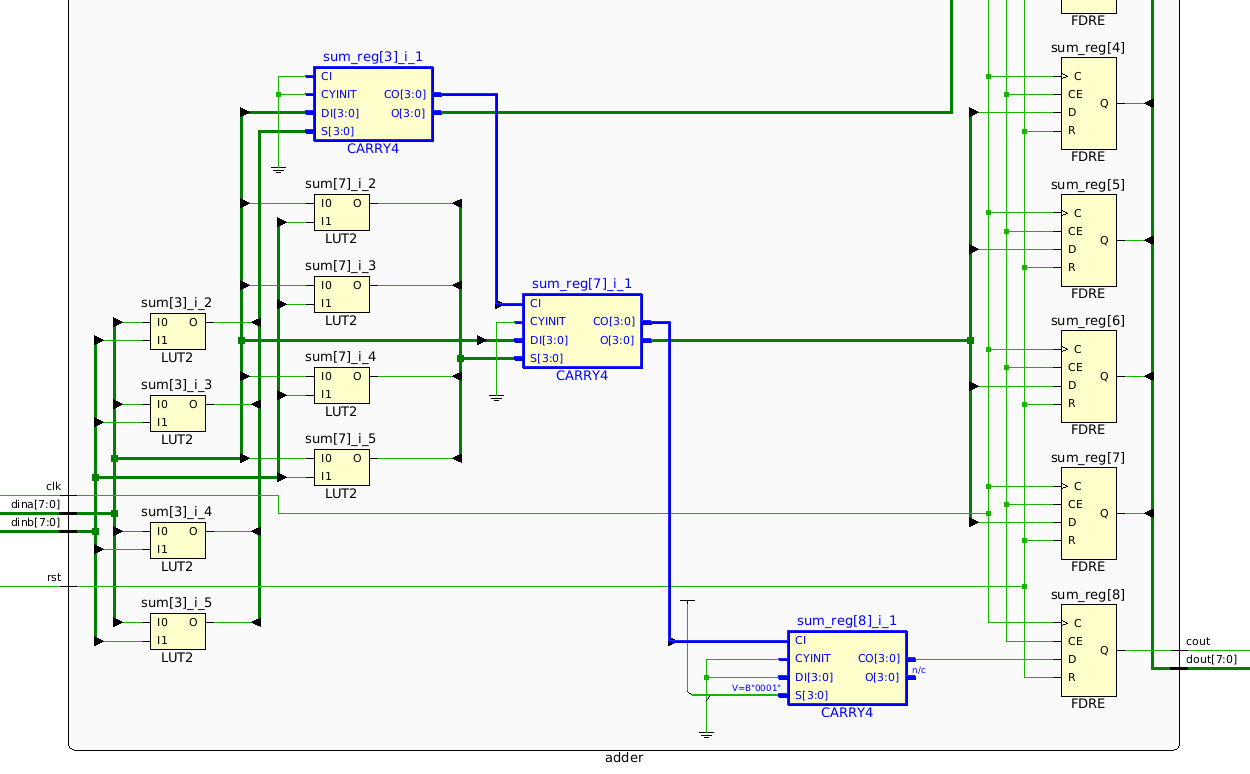
\includegraphics[valign=c, width=14.0cm]{figures/carry_chain_edif_3.png}
    \captionof{figure}{A \texttt{CARRY4} chain of size 3 as shown in the Vivado netlist viewer}
    \label{fig:carry_chain_edif}
}
\begin{multicols}{2}
\vspace{1.0cm}
.

\newpage
\subsection{DSP Slices}

\textbf{DSPs} \quad 
FPGAs are often used as low latency Digital Signal Processing (DSP) accelerators. 
Common DSP subsystems like Finite Impulse Response (FIR) filters, Fast Fourier Transform (FFTs), and convolutional neural nets (CNNs) demand fast large scale multiply-accumulate (MAC) capabilities. 
The 7-Series arhictecture integrates DSP BELs into the logic fabric called DSP48E1 that can facilitate MAC efficiently. 
The architecture hierarchy for DSPs is simple compared to CLBs and SLICEs. 
A \texttt{DSP48E1} Tile contains two \texttt{DSP48E1} Sites, each containing one \texttt{DSP48E1} BEL, which can host a \texttt{DSP48E1} Cell. 

{
    \centering
    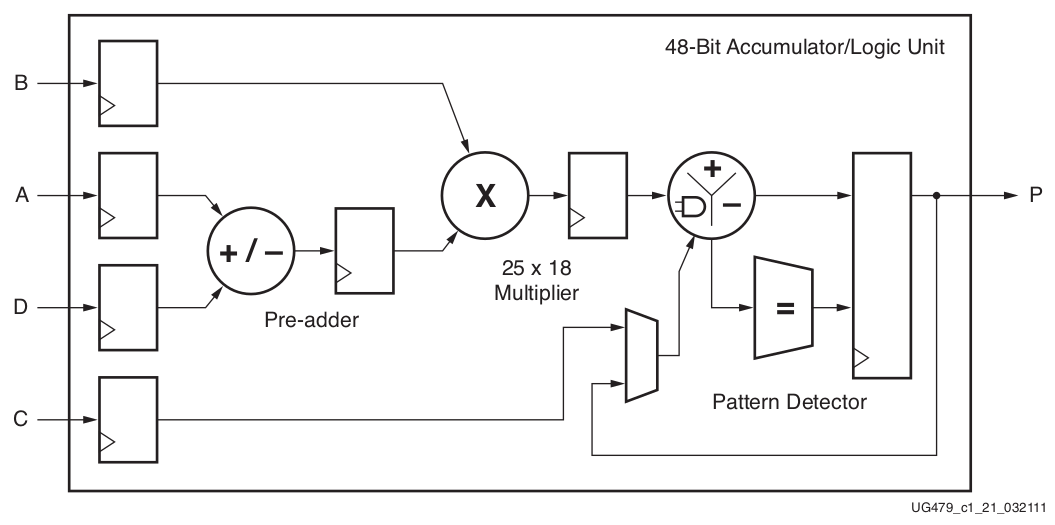
\includegraphics[width=\columnwidth]{figures/dsp_diagram.png}
    \captionof{figure}{
        Basic \texttt{DSP48E1} Slice Functionality
    }
    \label{dsp_diagram}
}
\vspace{0.5cm}

\textbf{DSP Cascades} \quad 
Higher level DSP functions are supported by cascading \texttt{DSP48E1} slices in a \texttt{DSP48E1} column.
Much like \texttt{CARRY4} chains, \texttt{DSP48E1} cascades must necessarily be placed vertically consecutively across \texttt{DSP48E1} Sites. 
They are connected by three busses: \texttt{ACOUT} to \texttt{ACIN}, \texttt{BCOUT} to \texttt{BCIN}, \texttt{PCOUT} to \texttt{PCIN}.
These signal busses run directly between the vertical \texttt{DSP48E1} slices without burdening the general routing resources. 
The ability to cascade this way provides a high-performance and low-power implementation of digital signal processing systems. 

\vspace{1.0cm}
{
    \centering
    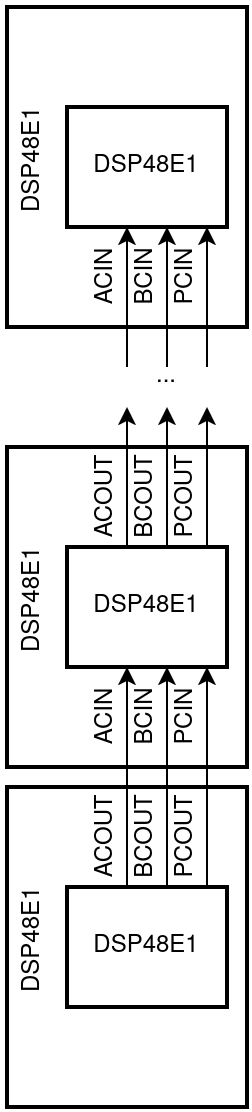
\includegraphics[valign=c, width=2.5cm]{figures/dsp_cascade_placement.png}
    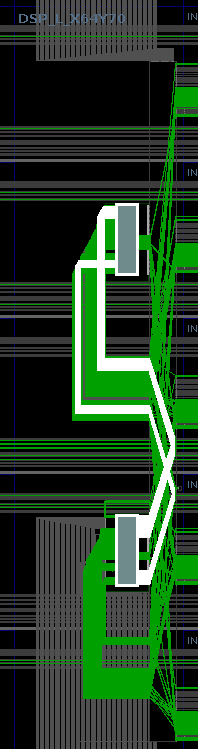
\includegraphics[valign=c, width=3.0cm]{figures/dsp_cascade_routed.png}
    \captionof{figure}{
        A \texttt{DSP48E1} cascade of size 2 placed across 2 \texttt{DSP48E1} Sites.
        \textbf{Left:} Simplified view, \textbf{Right:} As shown in the Vivado device viewer.
    }
}

\end{multicols}
{
    \centering
    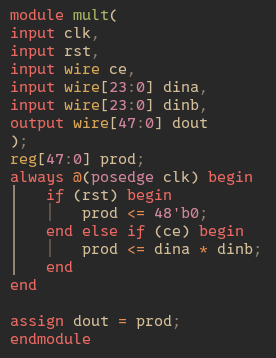
\includegraphics[valign=c, width=4.0cm]{figures/mult_synthesis.png}
    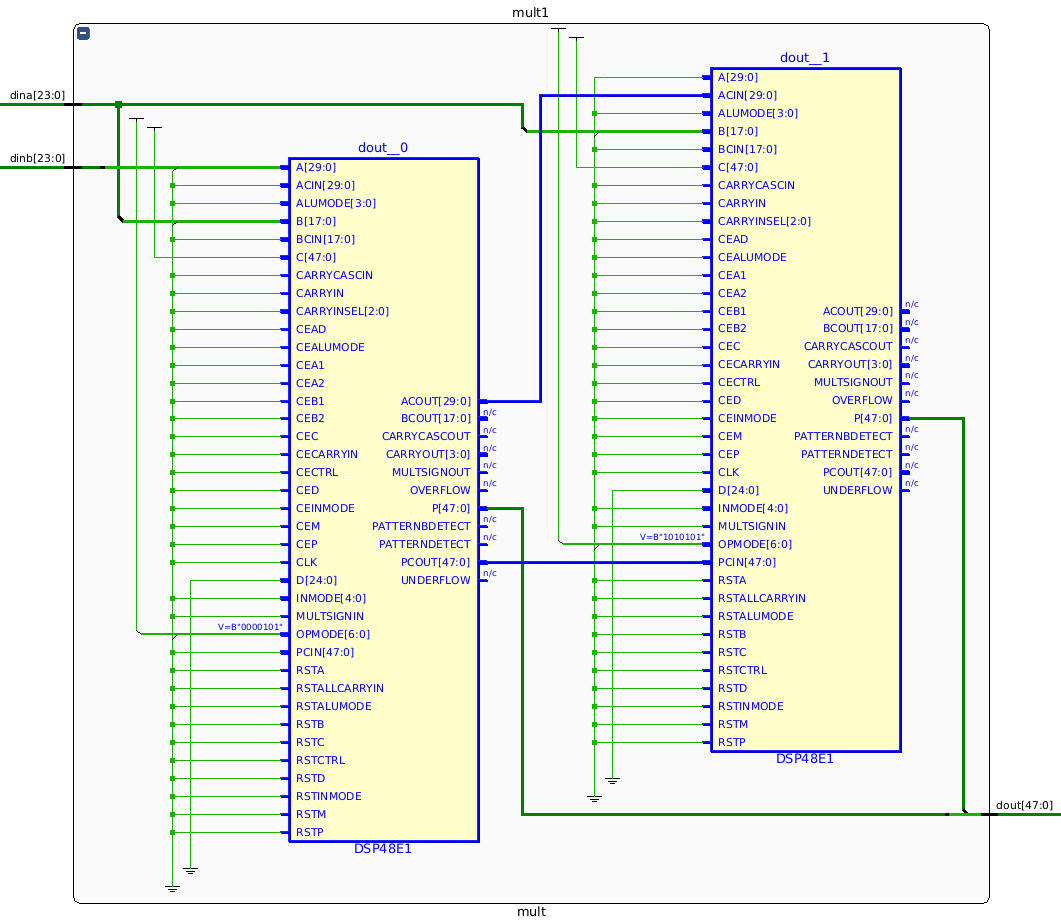
\includegraphics[valign=c, width=13.0cm]{figures/dsp_synthesis.png}
    \captionof{figure}{
        Simple multiplier synthesis from user design.
    }
    \label{mult_synthesis}
}
\begin{multicols}{2}


\newpage

\subsection{Block RAM}
In addition to SLICEs and DSPs, the 7-Series also offers dedicated Block Random Access Memory (BRAM) BELs. 
These BRAMs come in two variants: \textbf{RAMB18E1} and \textbf{RAMB36E1}. 
\begin{itemize}
\item \texttt{RAMB18E1} - 
Has a capacity of 18 Kilobits. 
It can be configured as single port RAM with dimensions ranging between (1-bit wide by 16K deep) to (18-bit wide by 1024 deep). 
It can also be configured as a (36-bit wide by 512 deep) true simple dual port RAM. 
\item \texttt{RAMB36E1} - 
Has a capacity of 36 Kilobits. 
It can be configured as single port RAM with dimensions ranging between (1-bit wide by 32K deep) to (36-bit wide by 1024 deep). 
It can also be configured as a (72-bit wide by 512 deep) simple dual port RAM. 
\end{itemize}

One BRAM Tile contains one \texttt{RAMB36E1} Site and two \texttt{RAMB18E1} Sites. 
The \texttt{RAMB36E1} Site contains one \texttt{RAMB36E1} BEL, which can host one \texttt{RAMB36E1} Cell. 
Likewise, the \texttt{RAMB18E1} Site contains one \texttt{RAMB18E1} BEL, which can host one \texttt{RAMB18E1} Cell. 

Like DSP cascades, BRAMs may also be cascaded together in a column to implement large memories efficiently, with some intermediate signals between them routed intra-Tile without burdening the general routing. 
However, unlike DSPs, large memories decomposed amongst multiple BRAMs can also be routed together through general routing. 
Furthermore, in most design scenarios, large memories will not utilize the intra-Tile signals. 

To simplify the problem space, we will not constrain large BRAMs to be cascaded together in consecutive vertical Tiles. 
We can essentially treat \texttt{RAMB18E1} and \texttt{RAMB36E1} Cells as loose, minimally constrained single cells, in contrast to the highly constrained \texttt{DSP48E1} cascades and \texttt{CARRY4} chains.

{
    \centering
    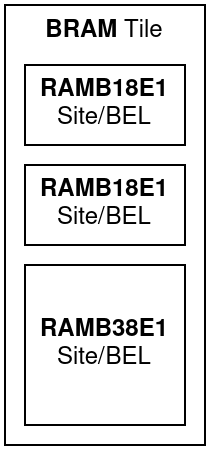
\includegraphics[valign=c, width=3.0cm]{figures/bram.png}
    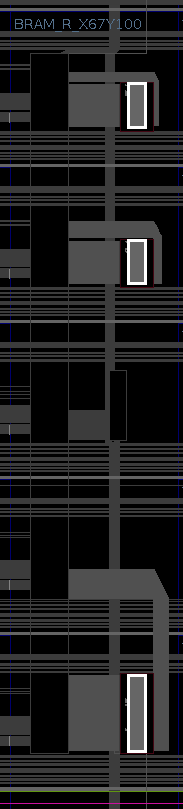
\includegraphics[valign=c, width=2.0cm]{figures/bram_tile.png}
    \captionof{figure}{
        A BRAM Tile containing two \texttt{RAMB18E1} Sites and one \texttt{RAMB36E1} Site.
        \textbf{Left:} simplified view. \textbf{Right:} as seen in the device viewer, BELs highlighted in white. 
    }
    \label{fig:bram_tile}
}

{
    \centering
    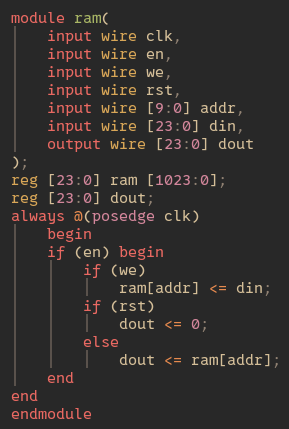
\includegraphics[valign=c, width=4.0cm]{figures/bram_synthesis.png}
    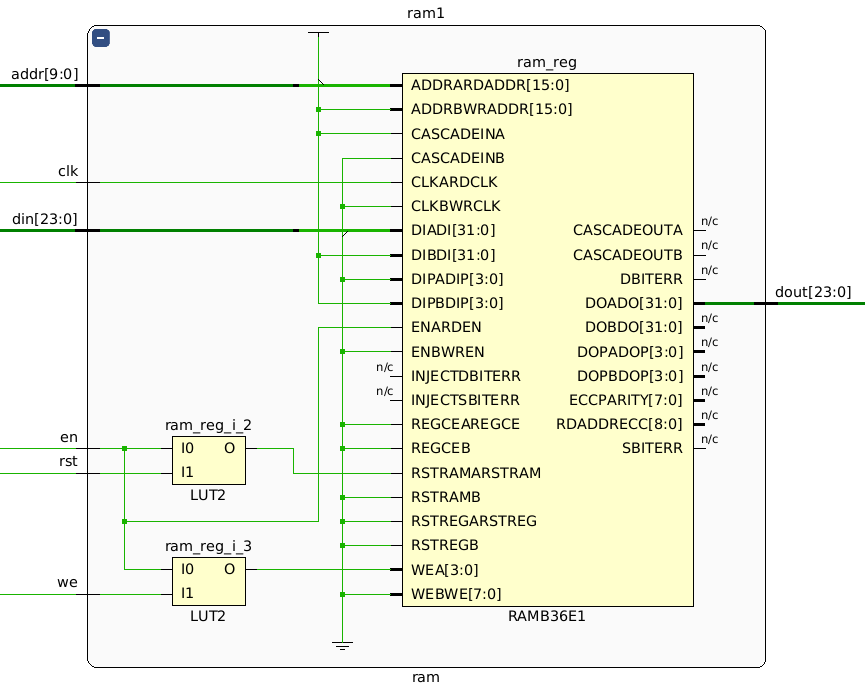
\includegraphics[valign=c, width=\columnwidth]{figures/bram_edif.png}
    \captionof{figure}{
        An example of BRAM synthesis (via inference)
    }
    \label{fig:bram_synthesis}
}

\subsection{Further Documentation}

For more in-depth details about 7-Series FPGAs, refer to the official Xilinx user guides such as:
\begin{itemize}
\item \emph{7 Series FPGAs Overview} (UG476)
\item \emph{7 Series FPGA Configurable Logic Block} (UG474)
\item \emph{7 Series Memory Resources} (UG473)
\item \emph{7 Series DSP48E1 Slice} (UG479)
\end{itemize}

This architectural context provides the necessary background for understanding how a placement algorithm should account for resource constraints and optimize performance in modern FPGA designs.



\newpage

\section{FPGA Design Flow and Toolchain}
\label{sec:fpga_flow_toolchain}

Modern FPGA designs require a sophisticated toolchain to bridge the gap between high-level hardware descriptions and the final bitstream used to configure the FPGA. 
Figure~\ref{fig:design_flow} illustrates a representative process that converts an abstract Hardware Description Language (HDL) design into a verified configuration file for a target device.

{
    \centering
    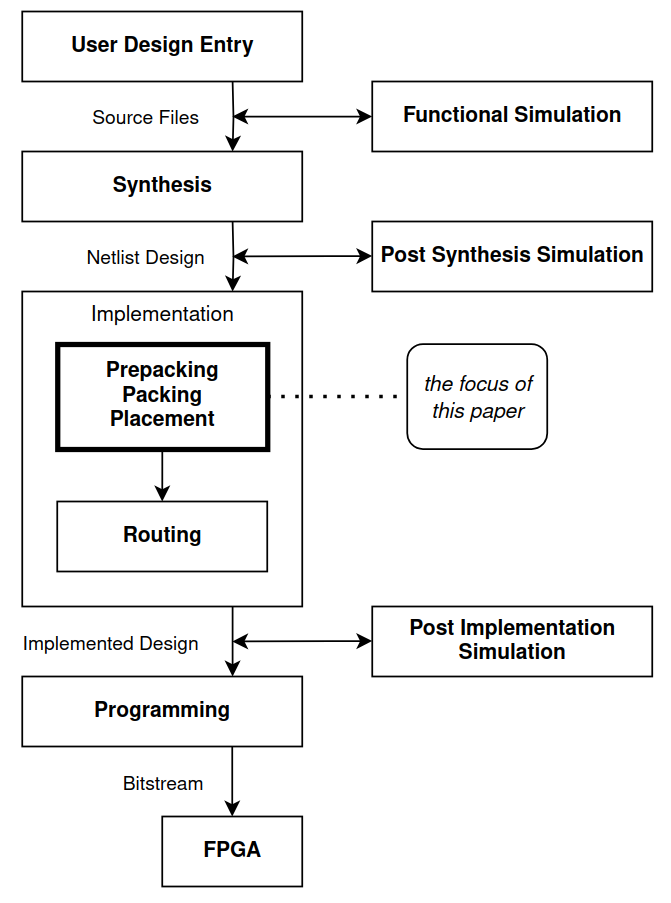
\includegraphics[width=0.9\columnwidth]{figures/design_flow.png}
    \captionof{figure}{A typical FPGA design and verification workflow.}
    \label{fig:design_flow}
}

\begin{enumerate}
\item \textbf{Design Entry:} 
    An engineer describes the intended functionality of the digital system using a hardware description language (HDL) such as Verilog or VHDL. 
    During this phase, the coding style can vary (behavioral, structural, dataflow, etc.), but it generally aims to capture high-level behavior rather than device-specific details.

\item \textbf{Synthesis:} 
    The synthesis tool parses the HDL source, performs logical optimizations, and maps the design onto primitive cells that suit the target FPGA technology. 
    The output is typically a structural \texttt{netlist} (e.g., EDIF or structural Verilog) which details how the design’s logic is broken down into LUTs, FFs, and other vendor-specific cells.

\item \textbf{Placement and Routing (Implementation):} 
    In \emph{placement}, each logical cell from the synthesized netlist is assigned to a physical location on the FPGA fabric. 
    For instance, LUTs and FFs go into specific \emph{BELs} within the device’s CLB sites, and specialized cells such as DSPs and Block RAMs must be placed in their corresponding tile types. 
    Next, \emph{routing} determines how signals are physically wired through the FPGA’s configurable interconnect network. 
    Modern tools often interleave these steps (e.g., fluid-placement routing or routing-aware placement) to better meet timing and area objectives.

\item \textbf{Bitstream Generation:} 
    After a design is fully placed, routed, and timing-closed, the toolchain produces a final \emph{bitstream} that sets the configuration of every programmable element in the FPGA. 
    This bitstream can then be loaded onto the device, either through vendor software or via a custom programming interface.

\item \textbf{Verification:} 
    In parallel to the design flow, simulations and testbenches validate correctness of the user's design at multiple abstraction levels. 
    Engineers may begin with behavioral simulations, then progress to post-synthesis simulations, and finally to post-implementation simulations that incorporate estimated routing delays. 
    With each higher level of fidelity, computational requirements grow significantly due to increasing complexity and the need to analyze more variables over time. 
    Ensuring correct functionality and meeting timing closure at the post-implementation stage is crucial before deploying the design to hardware. 
    Given the importance of thorough verification, many established companies dedicate one verification engineer for every design engineer.
\end{enumerate}

% This workflow underscores the critical role of \textbf{placement} in bridging the netlist to a physical realization. 
% An efficient placement algorithm can drastically reduce compile times and improve design performance, enabling broader adoption of FPGAs in application spaces that require fast design iteration.

\newpage

\section{RapidWright API}
\label{sec:rapidwright_api}

\textbf{RapidWright} is an open-source Java framework from AMD/Xilinx that provides direct access to the netlist and device databases used by vendor tools. 
This framework positions itself as an additional workflow column, allowing users to intercept or replace stages of the standard design flow with custom optimization stages (see Figure~\ref{fig:vivado_dcps}).

\begin{itemize}
\item \textbf{Design Checkpoints:} 
    RapidWright leverages \texttt{.dcp} files (design checkpoints) generated at various stages of a Vivado flow. 
    By importing a checkpoint, engineers can manipulate the netlist, placement, or routing externally, then re-export a modified checkpoint for further processing in the Vivado workflow column.

\item \textbf{Key Packages:} 
    RapidWright revolves around three primary data model packages:
    \begin{enumerate}
    \item \texttt{edif} -- Represents the logical netlist in an abstracted EDIF-like structure.
    \item \texttt{design} -- Contains data structures for the physical implementation (Cells, Nets, Sites, BELs, etc.).
    \item \texttt{device} -- Provides a database of the target FPGA architecture (e.g., Site coordinates, Tile definitions, routing resources).
    \end{enumerate}

\item \textbf{Interfacing with the Netlist and Device:} 
    An engineer can query the netlist to find specific resources (LUTs, FFs, DSPs, etc.) and then map or move them onto device sites. 
    This level of control over backend resources is necessary for research in custom placement, advanced packing techniques, or experimental routing algorithms.
\end{itemize}

{
    \centering
    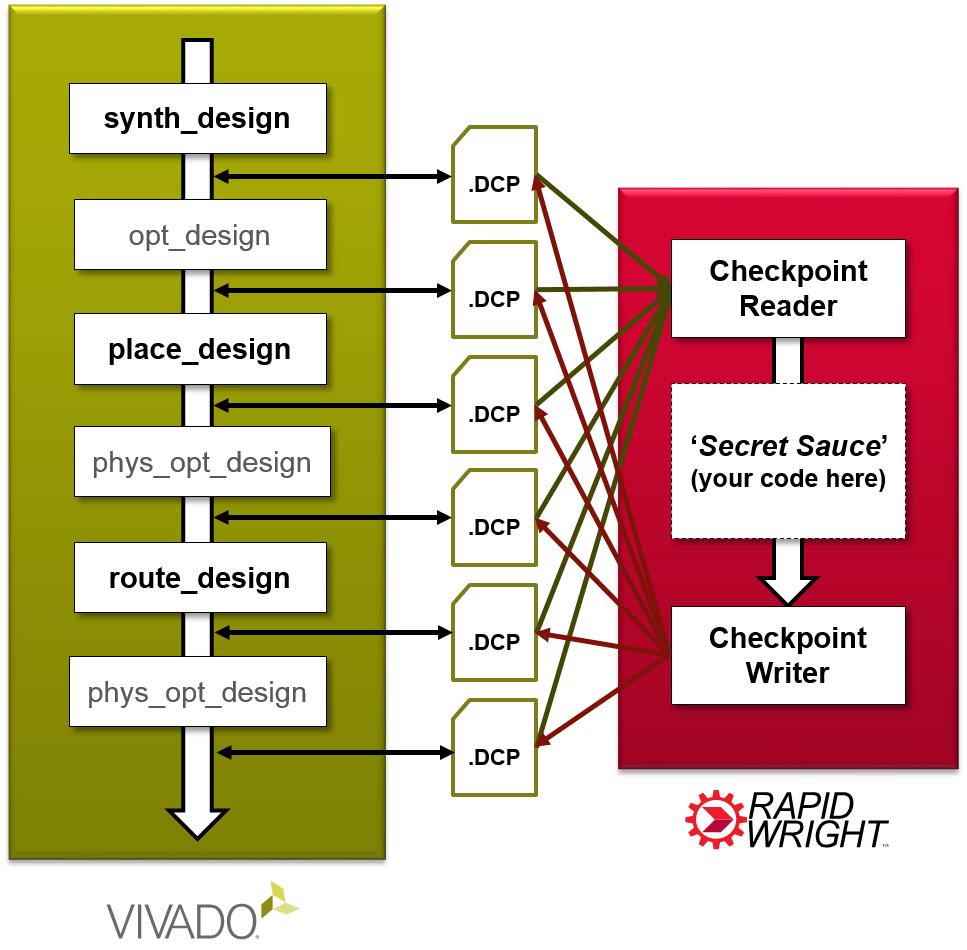
\includegraphics[width=0.8\columnwidth]{figures/vivado_dcps.png}
    \captionof{figure}{RapidWright workflow integrating into the default Vivado design flow.}
    \label{fig:vivado_dcps}
}

By exposing these low-level internals, RapidWright allows fine-grained design transformations that go beyond the standard Vivado IDE’s capabilities. 
Researchers can prototype new EDA strategies without needing to re-implement an entire FPGA backend from scratch, thus accelerating innovation in placement and routing methodologies.

\subsection{What is a Netlist?}
\label{subsec:netlist}
In its most general form, a netlist is a list of every component in an electronic design paired with a list of nets they connect to. 
Depending on the abstraction level at hand, these components can be transistors, logic gates, macrocells, or increasingly higher-level modules. 
Generally, a net denotes any group of two or more interconnected components.
In an electronics context, a net can be though of as a wire connecting multiple pins between multiple components, with each wire having one voltage source and one or more voltage sinks. 
Thus, one could express the netlist as a hypergraph, nodes representing components, hyperedges representing wires connecting two or more component. 
More precisely, these hyperedges connect the ports on the components, not the components themselves, with each component exposing multiple ports. 

In FPGA context, the components are logical cells (\texttt{LUTs}, \texttt{CARRY4s}, etc.) or hierarchical cells (Verilog module instances) with pins connected together by wires. 
In Vivado, a Netlist can be synthesized as a Hierarchical or a Flattened netlist. 
Figure ~\ref{fig:hierarchical_design} shows an example a Verilog design with modules instantiated in a hierarchy. 
Figure ~\ref{fig:hier_netlist} shows the design synthesized into a \textbf{hierarchical netlist} with \textbf{hierarchical cells} and \textbf{leaf cells}. 
The synthesizer attempts to construct the module hierarchy as close to the module instantiation hierarchy defined by the user design entry. 
Figure ~\ref{fig:flat_netlist} shows the same design but synthesized into a \textbf{flattened netlist} containing \textbf{only leaf cells}. 

In either synthesized netlist, the \textbf{leaf cells}, (deepest level cells), must necessarily consist only of \textbf{primitive cells} from the architecture's primitive cell library (\texttt{LUT6}, \texttt{FDRE}, \texttt{CARRY4}, \texttt{DSP48E1}, etc.). 
The netlist can be compiled and exported as a purely structural low-level Verilog file, or an Electrinic Design Interchange Format (EDIF) file, both describing the netlist explicitly as a list of cell instances connected by a list of wires. 

\newpage
\end{multicols}
{
    \raggedright
    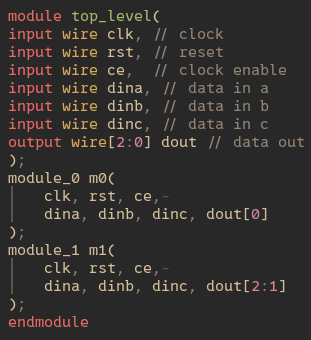
\includegraphics[valign=t, scale=0.3]{figures/netlist_synth/top_level.png}
    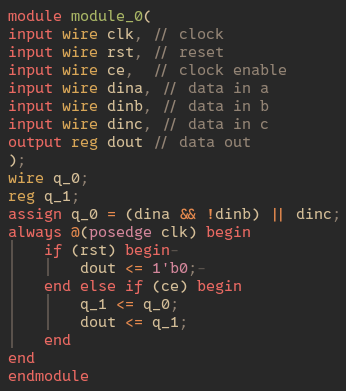
\includegraphics[valign=t, scale=0.3]{figures/netlist_synth/module_0.png}
    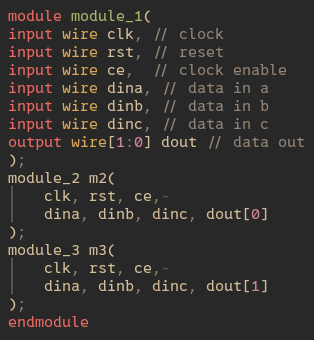
\includegraphics[valign=t, scale=0.3]{figures/netlist_synth/module_1.png}
    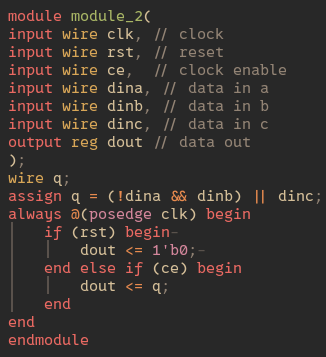
\includegraphics[valign=t, scale=0.3]{figures/netlist_synth/module_2.png}
    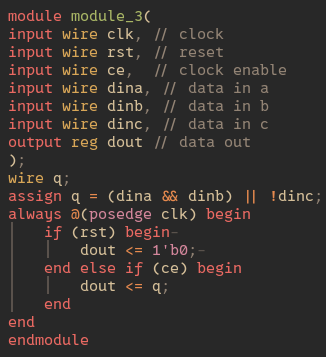
\includegraphics[valign=t, scale=0.3]{figures/netlist_synth/module_3.png}
    \captionof{figure}{A simple HDL design with module hierarchy.}
    \label{fig:hierarchical_design}
}
\vspace{0.5cm}
{
    \centering
    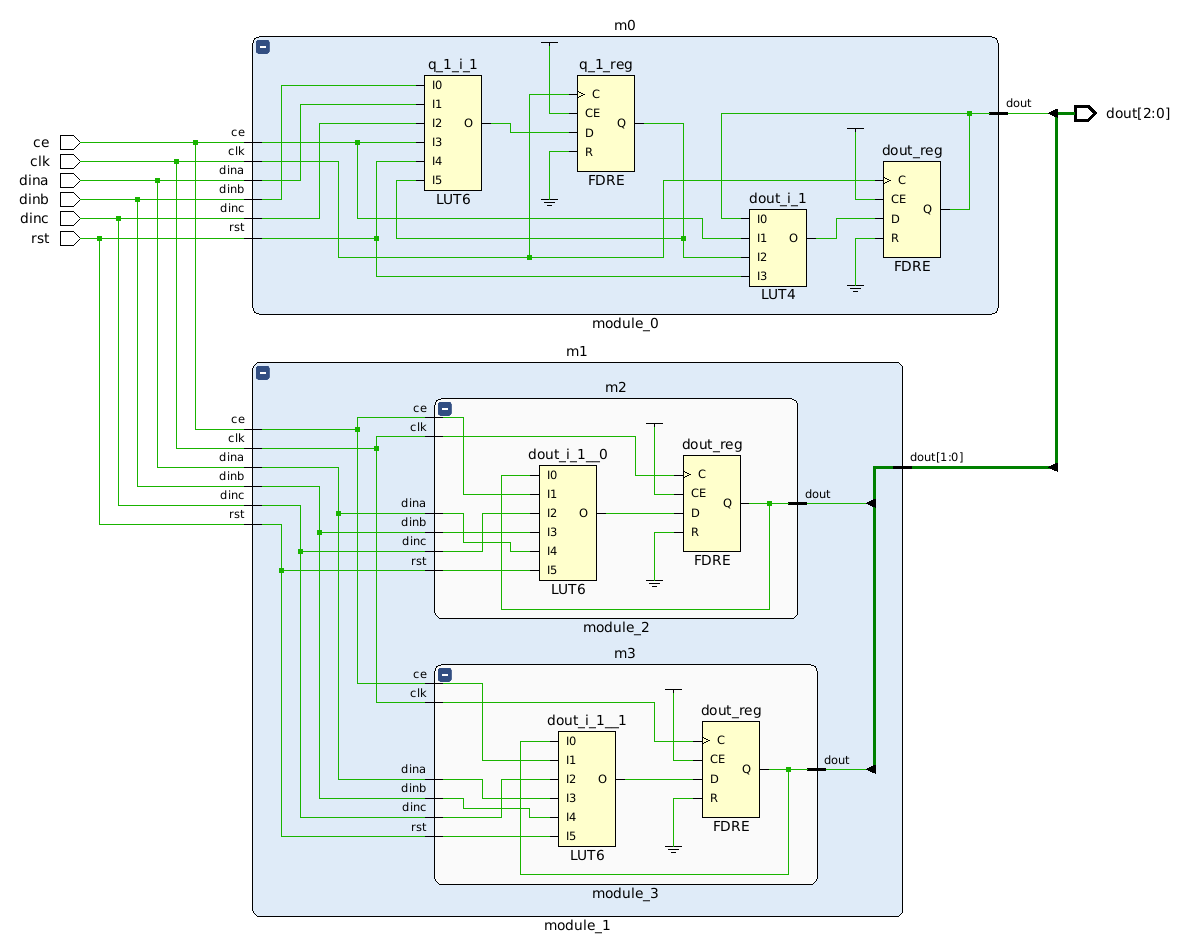
\includegraphics[valign=c, width=11.5cm]{figures/netlist_synth/hier_netlist.png}
    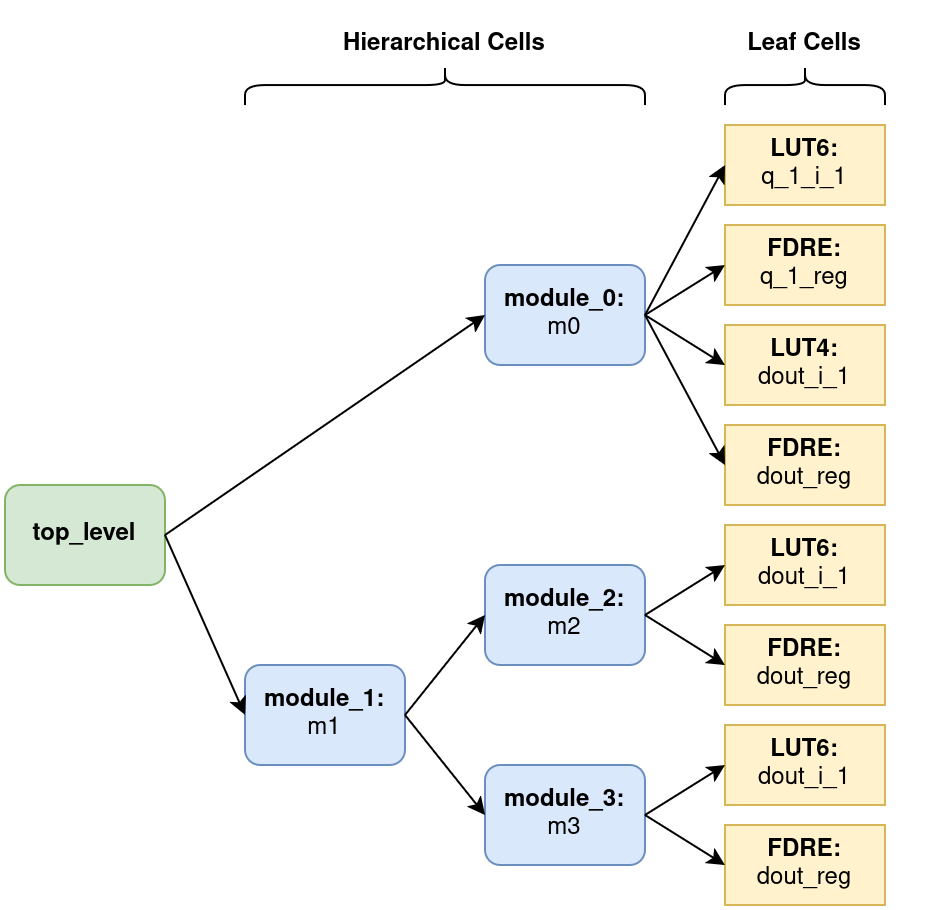
\includegraphics[valign=c, width=6cm]{figures/netlist_synth/hier_graph.png}
    \captionof{figure}{
        \textbf{Left:} A hierarchical netlist consisting of LUTs and FFs.
        \textbf{Right:} The cell hierarchy tree.
    }
    \label{fig:hier_netlist}
}
\vspace{0.5cm}
{
    \centering
    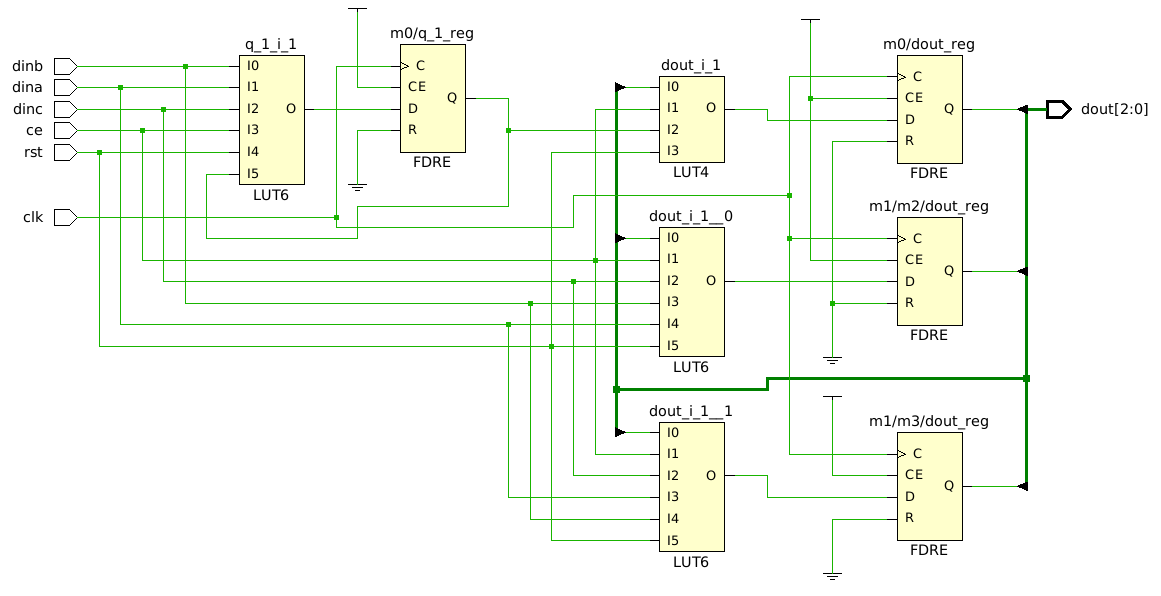
\includegraphics[valign=c, width=13.0cm]{figures/netlist_synth/flat_netlist.png}
    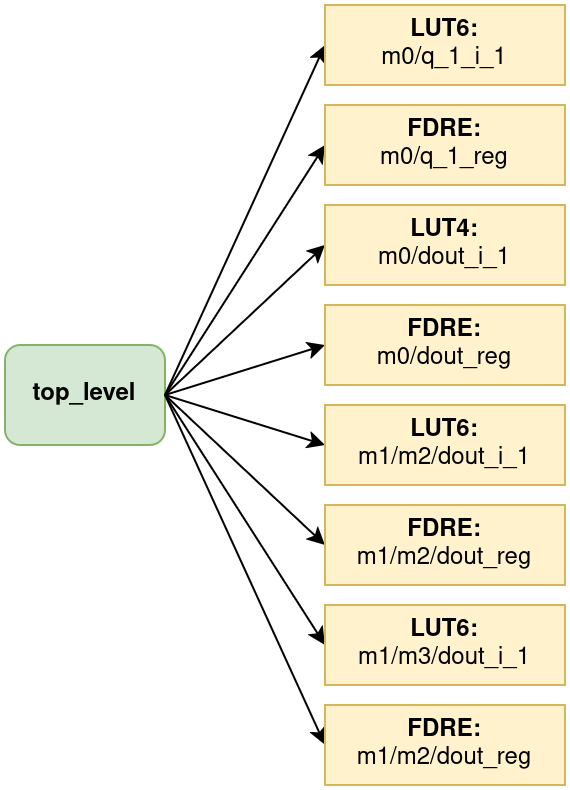
\includegraphics[valign=c, width=4cm]{figures/netlist_synth/flat_graph.png}
    \captionof{figure}{
        \textbf{Left:} A flattened netlist consisting of LUTs and FFs.
        \textbf{Right:} The flattened cell hierarchy tree.
    }
    \label{fig:flat_netlist}
}
\newpage
\begin{multicols}{2}

\subsection{Netlist Traversal and Manipulation via RapidWright}

RapidWright represents the logical netlist objects via the \texttt{edif} classes:
\begin{itemize}
    \item \texttt{EDIFNetlist}: The full logical netlist of a \texttt{Design}. 
    \item \texttt{EDIFNet}: A logical net within an \texttt{EDIFNetlist}.
    \item \texttt{EDIFHierNet}: Combines an \texttt{EDIFNet} with a full hierarchical instance name to uniquely identify a net in a netlist.
    \item \texttt{EDIFCell}: A logical cell in an \texttt{EDIFNetlist}. 
    \item \texttt{EDIFCellInst}: An instance of an \texttt{EDIFCell}. 
    \item \texttt{EDIFHierCellInst}: An \texttt{EDIFCellInst} with its hierarchy, described by all the \texttt{EDIFCellInst}s that sit above it within the netlist.
    \item \texttt{EDIFPort}: A port on an \texttt{EDIFCell}. 
    \item \texttt{EDIFPortInst}: An instance of a port on an \texttt{EDIFCellInst}. 
    \item \texttt{EDIFHierPortInst}: Combines an \texttt{EDIFPortInst} with a full hierarchical instance name to uniquely identify a port instance in a netlist. 
\end{itemize}


Using these classes and their associated methods, we can traverse the logical netlist (\texttt{EDIFNetlist}) and analyze or manipulate it as we see fit. 
A netlist can be easily extracted from a \texttt{.dcp} design checkpoint file and traversed like shown in Listing \ref{lst:netlist_extract}. 
This is performed on the same design shown in figure \ref{fig:flat_netlist}.

\begin{lstlisting}[language=java, caption={Basic netlist extraction and traversal}, label={lst:netlist_extract}]
Design design = Design.readCheckpoint("synth.dcp")
EDIFNetlist netlist = design.getNetlist();

// Example task:
// Extract the set of all unique nets from the design.

// Initialize a new Set:
Set<EDIFNet> netSet = new HashSet<>();

// Access all leaf cells
List<EDIFCellInst> ecis = netlist.getAllLeafCellInstances();

// Traverse the cell list
for (EDIFCellInst eci : ecis) {
    // Access the ports on this cell
    Collection<EDIFPortInst> epis = eci.getPortInsts();
    for (EDIFPortInst epi : epis) {
        // Access the net on this port
        EDIFNet net = epi.getNet();
        netSet.add(net);
    }
}

// Downstream task:
// For each unique net, print out the incident cells.

// Traverse the set of nets
for (EDIFNet net : netSet) {
    System.out.println("Net: " + net.getName());
    // Access the ports connected to this net
    Collection<EDIFPortInst> epis = net.getPortInsts();
    for (EDIFPortInst epi : epis) {
        // Access the cell that this port belongs to
        EDIFCellInst eci = epi.getCellInst();
        if (eci == null) {
            // (top_level ports have no associated cell)
            continue;
        } else {
            System.out.println(
                "\tCell: " + eci.getName() + 
                ",\tCellType: " + eci.getCellName()
            );
        }
    }
}
\end{lstlisting}

{
    \centering
    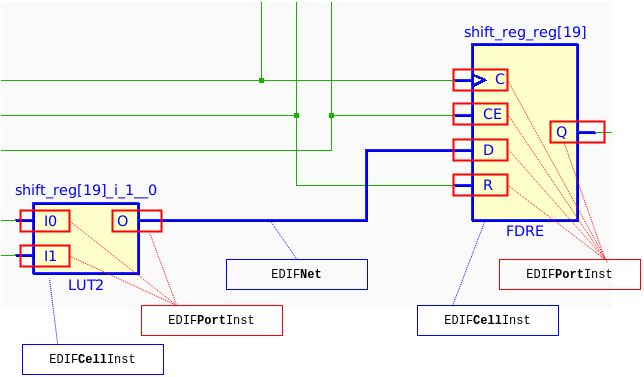
\includegraphics[valign=c, width=\columnwidth]{figures/traversal.png}
    \captionof{figure}{\texttt{Netlist} traversal via the \texttt{EDIFCellInst}, \texttt{EDIFPortInst}, and \texttt{EDIFNet} classes}
    \label{fig:traversal}
}
\vspace{0.5cm}

In this method, we get the list of all \texttt{EDIFCellInst} from the \texttt{EDIFNetlist} and traverse the list of cells and access their connected nets. 
Alternatively, we could have also extracted the list of all \texttt{EDIFNet}s directly from the \texttt{design} and traversed the nets to access their connected cells. 

\begin{lstlisting}[caption={Code Printout}]
Net: dout[0]
	Port: I0, Cell: dout_i_1, CellType: LUT4
	Port: Q, Cell: m0/dout_reg, CellType: FDRE
Net: q_1
	Port: I2, Cell: dout_i_1, CellType: LUT4
	Port: Q, Cell: m0/q_1_reg, CellType: FDRE
	Port: I5, Cell: q_1_i_1, CellType: LUT6
Net: ce
	Port: I1, Cell: dout_i_1, CellType: LUT4
	Port: I1, Cell: dout_i_1__0, CellType: LUT6
	Port: I1, Cell: dout_i_1__1, CellType: LUT6
	Port: I3, Cell: q_1_i_1, CellType: LUT6
Net: dout[1]
	Port: I0, Cell: dout_i_1__0, CellType: LUT6
	Port: Q, Cell: m1/m2/dout_reg, CellType: FDRE
Net: dout_i_1__1_n_0
	Port: O, Cell: dout_i_1__1, CellType: LUT6
	Port: D, Cell: m1/m3/dout_reg, CellType: FDRE
Net: clk
	Port: C, Cell: m0/dout_reg, CellType: FDRE
	Port: C, Cell: m0/q_1_reg, CellType: FDRE
	Port: C, Cell: m1/m2/dout_reg, CellType: FDRE
	Port: C, Cell: m1/m3/dout_reg, CellType: FDRE
Net: dout[2]
	Port: I0, Cell: dout_i_1__1, CellType: LUT6
	Port: Q, Cell: m1/m3/dout_reg, CellType: FDRE
Net: <const0>
	Port: G, Cell: GND, CellType: GND
	Port: R, Cell: m0/dout_reg, CellType: FDRE
	Port: R, Cell: m0/q_1_reg, CellType: FDRE
	Port: R, Cell: m1/m2/dout_reg, CellType: FDRE
	Port: R, Cell: m1/m3/dout_reg, CellType: FDRE
Net: <const1>
	Port: P, Cell: VCC, CellType: VCC
	Port: CE, Cell: m0/dout_reg, CellType: FDRE
	Port: CE, Cell: m0/q_1_reg, CellType: FDRE
	Port: CE, Cell: m1/m2/dout_reg, CellType: FDRE
	Port: CE, Cell: m1/m3/dout_reg, CellType: FDRE
Net: dout_i_1__0_n_0
	Port: O, Cell: dout_i_1__0, CellType: LUT6
	Port: D, Cell: m1/m2/dout_reg, CellType: FDRE
Net: rst
	Port: I3, Cell: dout_i_1, CellType: LUT4
	Port: I5, Cell: dout_i_1__0, CellType: LUT6
	Port: I5, Cell: dout_i_1__1, CellType: LUT6
	Port: I4, Cell: q_1_i_1, CellType: LUT6
Net: dinc
	Port: I2, Cell: dout_i_1__0, CellType: LUT6
	Port: I2, Cell: dout_i_1__1, CellType: LUT6
	Port: I2, Cell: q_1_i_1, CellType: LUT6
Net: dinb
	Port: I3, Cell: dout_i_1__0, CellType: LUT6
	Port: I4, Cell: dout_i_1__1, CellType: LUT6
	Port: I0, Cell: q_1_i_1, CellType: LUT6
Net: dina
	Port: I4, Cell: dout_i_1__0, CellType: LUT6
	Port: I3, Cell: dout_i_1__1, CellType: LUT6
	Port: I1, Cell: q_1_i_1, CellType: LUT6
Net: q_1_i_1_n_0
	Port: D, Cell: m0/q_1_reg, CellType: FDRE
	Port: O, Cell: q_1_i_1, CellType: LUT6
Net: dout_i_1_n_0
	Port: O, Cell: dout_i_1, CellType: LUT4
	Port: D, Cell: m0/dout_reg, CellType: FDRE
\end{lstlisting}


\subsection{Placement Flow via RapidWright}
\label{subsec:placement}
\end{multicols}
{
    \centering
    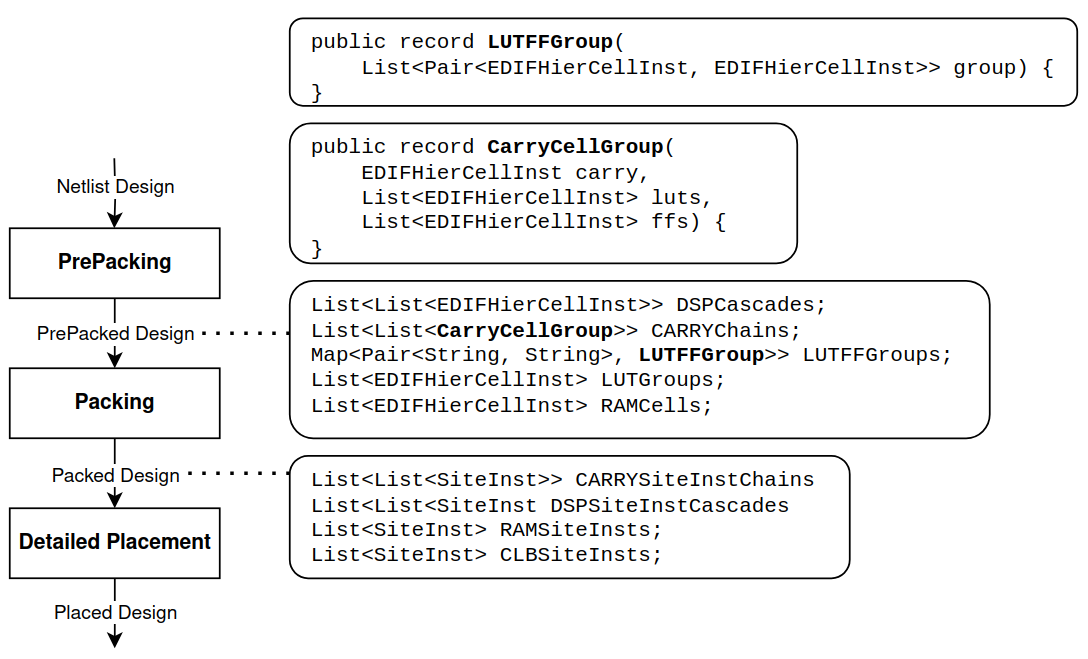
\includegraphics[width=0.8\columnwidth]{figures/substages.png}
    \captionof{figure}{The data classes populated at each substage: \texttt{PrepackedDesign}, \texttt{PackedDesign}, and \texttt{PlacedDesign}.}
    \label{fig:substages}
}
\begin{multicols}{2}
\label{sec:simulated_annealing}
With a basic understanding of FPGA architecture, design placement, and RapidWright, we have all the necessary pieces to implement our SA placer. 
Here we outline in detail each substage of our implementation: PrePacking, Packing, and Placement. 
Shown in Figure \ref{fig:edif_design_device} is an overview of the placement workflow. 
Figure \ref{fig:substages} shows the data structures of RapidWright objects that are populated at each stage: \texttt{PrepackedDesign}, which is a group of data structures around \texttt{EDIFHierCellInst}s, \texttt{PackedDesign}, which is a group fo data structures around \texttt{SiteInst}s, and finally, \texttt{PlacedDesign}, which is simply captured by the final RapidWright \texttt{Design} object. 

\vspace{0.5cm}
{
    \centering
    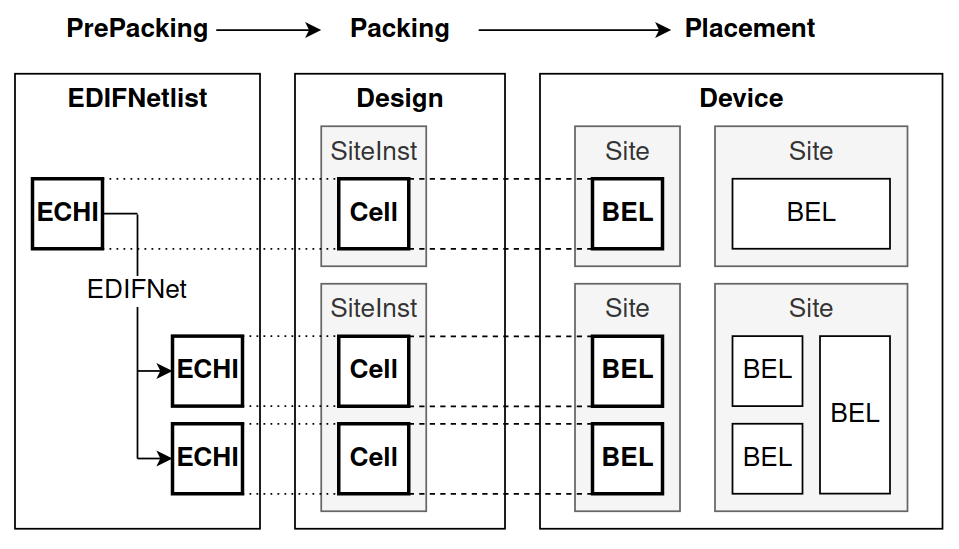
\includegraphics[width=0.9\columnwidth]{figures/edif_design_device.png}
    \captionof{figure}{Our placement workflow}
    \label{fig:edif_design_device}
}







\section{Prepacking}
\label{sec:prepacking}


The first step in our placement flow is \textbf{prepacking}. 
Recall from the 7-Series architecture that there are certain multi-cell structures that must adhere to certain placements constraints to ensure legality, and by design, to minimize wirelength. 
The job of the prepacker is to traverse the raw EDIF netlist, detect these multi-cell structures, and consolidate these cells into clusters or groups of clusters that naturally reflect these placement constraints. 

Recall that \texttt{CARRY4} chains must necessarily be placed vertically and consecutively across a column of SLICEs in ascending order. 
Likewise, \texttt{DSP48E1} cascades must necessarily be placed vertically and consecutively across a column of \texttt{DSP48E1} Sites in ascending order. 
A LUT-FF pair may be placed freely, but should be placed in the same lane within the same SLICE to minimize wirelength.

The raw EDIF netlist only tells us the list of nets and the cell ports that they connect to. 
It does not report the presence of any multi-cell structures (\texttt{CARRY4} chains, etc.). 
Thus, we must traverse the netlist to detect these multi-cell structures and store that structure information in a class we will call \texttt{PrepackedDesign}.

The code snippet in \ref{lst:carry_chains} shows how one can detect and collect these \texttt{CARRY4} chains using RapidWright. 
We first collect the cells in the design that are of type \texttt{CARRY4}, then iteratively traverse their Carry-Out (\texttt{CO}) to Carry-In (\texttt{CI}) nets to find incident \texttt{CARRY4} cells.
Each \texttt{CARRY4} chain has an anchor cell and a tail cell where the chain terminates.
The anchor is found when the \texttt{CI} net connects to Ground (\texttt{GND}), while the tail is found when the \texttt{CO} port is null. 
We can further detect if there are \texttt{LUT}s or \texttt{FF}s connected to the \texttt{CARRY4} cell and store that information in a data structure we will call \texttt{CarryCellGroup} as defined in figure \ref{fig:substages}.
This will help us in knowing which cells can be packed together into the same \texttt{Site} in the subsequent stages. 

Similarly, \texttt{DSP48E1} cascades can be found and collected by traversing the \texttt{PCOUT} \texttt{ACOUT} and \texttt{BCOUT} nets.
\texttt{LUT-FF} pairs can be found by inspecting the LUT output (O) net and checking for FF input (DI) ports. 
We can bucket these LUT-FF pairs by finding the set of unique \texttt{CE} \texttt{SR} net pairs to know which group of LUT-FF pairs can be placed within the same \texttt{Site}. 

The overall goal of prepacking is to detect the presence of these multi-cellular structures and consolidate that information into our \texttt{PrepackedDesign} object in preparation for the following Packing stage. 


\end{multicols}
{
    \centering
    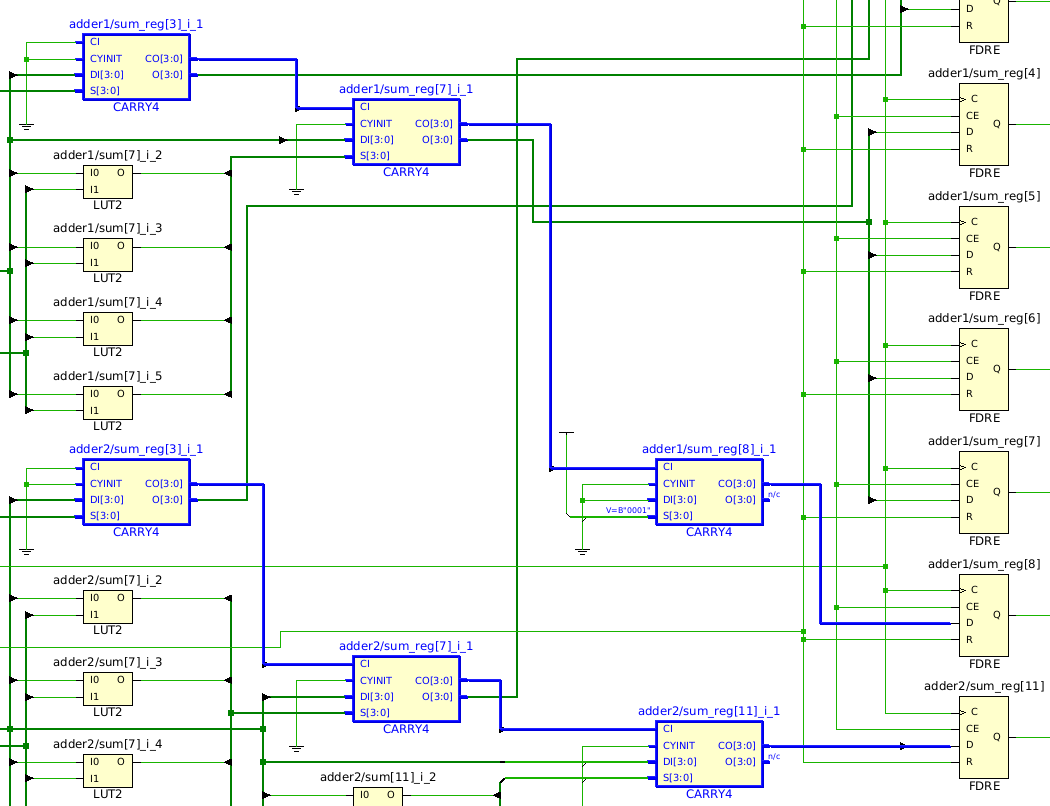
\includegraphics[width=0.8\columnwidth]{figures/carry_chain_traversal.png}
    \captionof{figure}{A netlist with two \texttt{CARRY4} chains, each of size 3}
    \label{fig:carry_chain_traversal}
}
\begin{multicols}{2}

\begin{lstlisting}[language=java, caption={Finding and storing carry chains.}, label={lst:carry_chains}]
Design design = Design.readCheckpoint("synth.dcp")
EDIFNetlist netlist = design.getNetlist();
List<EDIFCellInst> ecis = netlist.getAllLeafCellInstances();

// Select only the carry cells.
List<EDIFCellInst> carryCells = new ArrayList<>();
for (EDIFCellInst eci : ecis) {
    if (eci.getCellName().equals("CARRY4"))
        carryCells.add(eci);
}

// Find and remove carry chains until the list is empty
List<List<EDIFCellInst>> carryChains = new ArrayList<>();
while (!carryCells.isEmpty()) {
    // Set "currentCell" pointer to an arbitrary cell in list
    EDIFCellInst currentCell = carryCells.get(0);

    // Find this carry chain anchor.
    // Traverse the Carry-In (CI) to Carry-Out (CO) nets.
    // Anchor is found when net on the CI Port is Ground.
    while (true) {
        System.out.println(currentCell);
        // Access the CI port on this cell.
        EDIFPortInst sinkPort = currentCell.getPortInst("CI");
        // Access the net on this CI port.
        EDIFNet net = sinkPort.getNet();
        if (net.isGND()) {
            break; // Found this chain anchor!
        }
        // Get all ports on this net.
        List<EDIFPortInst> netPorts = net.getPortInsts();
        for (EDIFPortInst netPort : netPorts) {
            // Access the port belonging to another carry cell.
            EDIFCellInst sourceCell = netPort.getCellInst();
            if (sourceCell.getCellName().equals("CARRY4")) {
                // Move the "currentCell" pointer
                currentCell = sourceCell;
                break;
            }
        }
    }

    // Now currentCell points at this chain's anchor.

    // Now traverse in the opposite direction to find the chain tail.
    // Tail is found when the CO Port is null.
    // Collect the chain cells into an ordred list.
    List<EDIFCellInst> currentChain = new ArrayList<>();
    currentChain.add(currentCell);
    while (true) {
        EDIFPortInst sourcePort = currentCell.getPortInst("CO[3]");
        if (sourcePort == null) {
            break; // Found this chain's tail!
        }
        EDIFNet net = sourcePort.getNet();
        List<EDIFPortInst> netPorts = net.getPortInsts();
        for (EDIFPortInst netPort : netPorts) {
            EDIFCellInst sinkCell = netPort.getCellInst();
            if (netPort.getName().equals("CI") &&
                    sinkCell.getCellName().equals("CARRY4")) {
                currentCell = sinkCell;
                // Add the cell to the chain list.
                currentChain.add(currentCell);
                break;
            }
        }
    }
    // Add currentChain to the list of chains
    carryChains.add(currentChain);
    // Remove currentChain from the list of cells
    carryCells.removeAll(currentChain);
} // end while()

// Print out the carry chains. 
for (List<EDIFCellInst> chain : chains) {
    for (int i = 0; i < chain.size(); i++) {
        EDIFCellInst carry = chain.get(i);
        if (i == 0) {
            writer.write("\nAnchor Cell: " + carry.getName() + 
                ", CellType: " + carry.getCellName());
        } else {
            writer.write("\n\tCell: " + carry.getName() + 
                ", CellType: " + carry.getCellName());
        }
    }
}
\end{lstlisting}

\end{multicols}
\begin{lstlisting}[caption={Code Printout}]
Anchor Cell: adder2/sum_reg[3]_i_1, CellType: CARRY4
	Cell: adder2/sum_reg[7]_i_1, CellType: CARRY4
	Cell: adder2/sum_reg[11]_i_1, CellType: CARRY4
Anchor Cell: adder1/sum_reg[3]_i_1, CellType: CARRY4
	Cell: adder1/sum_reg[7]_i_1, CellType: CARRY4
	Cell: adder1/sum_reg[8]_i_1, CellType: CARRY4
\end{lstlisting}
\begin{multicols}{2}


\section{Placement}
\end{multicols}
{
    \centering
    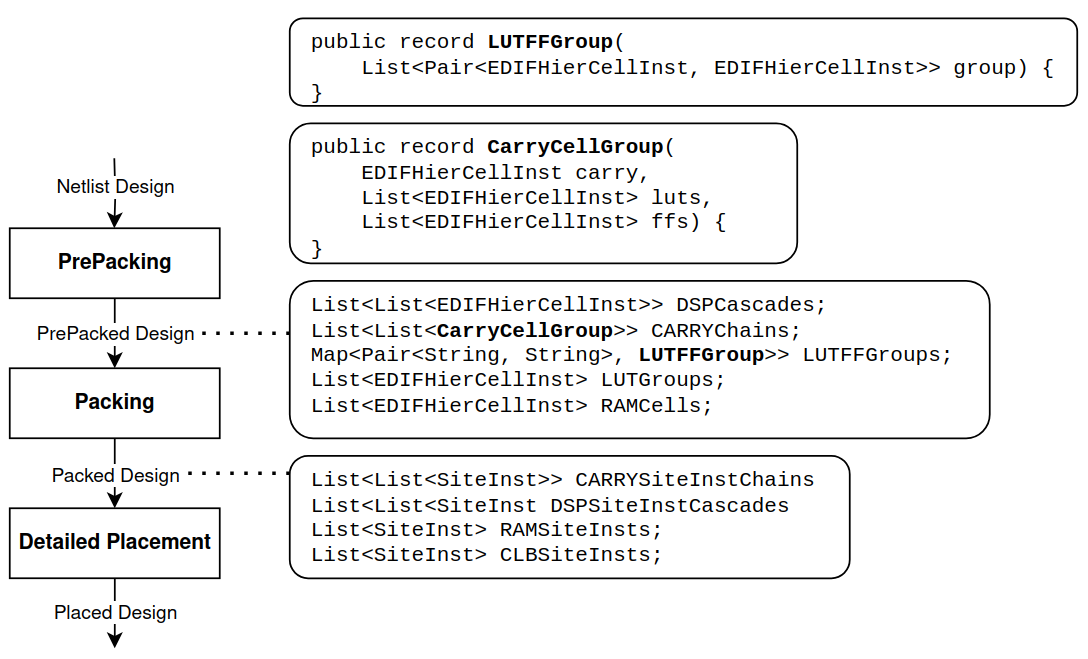
\includegraphics[width=0.8\columnwidth]{figures/substages.png}
    \captionof{figure}{The data classes populated at each substage: \texttt{PrepackedDesign}, \texttt{PackedDesign}, and \texttt{PlacedDesign}.}
    \label{fig:substages}
}
\begin{multicols}{2}
\label{sec:simulated_annealing}
With a basic understanding of FPGA architecture, design placement, and RapidWright, we have all the necessary pieces to implement our SA placer. 
Here we outline in detail each substage of our implementation: PrePacking, Packing, and Placement. 
Shown in Figure \ref{fig:edif_design_device} is an overview of the placement workflow. 
Figure \ref{fig:substages} shows the data structures of RapidWright objects that are populated at each stage: \texttt{PrepackedDesign}, which is a group of data structures around \texttt{EDIFHierCellInst}s, \texttt{PackedDesign}, which is a group fo data structures around \texttt{SiteInst}s, and finally, \texttt{PlacedDesign}, which is simply captured by the final RapidWright \texttt{Design} object. 

\vspace{0.5cm}
{
    \centering
    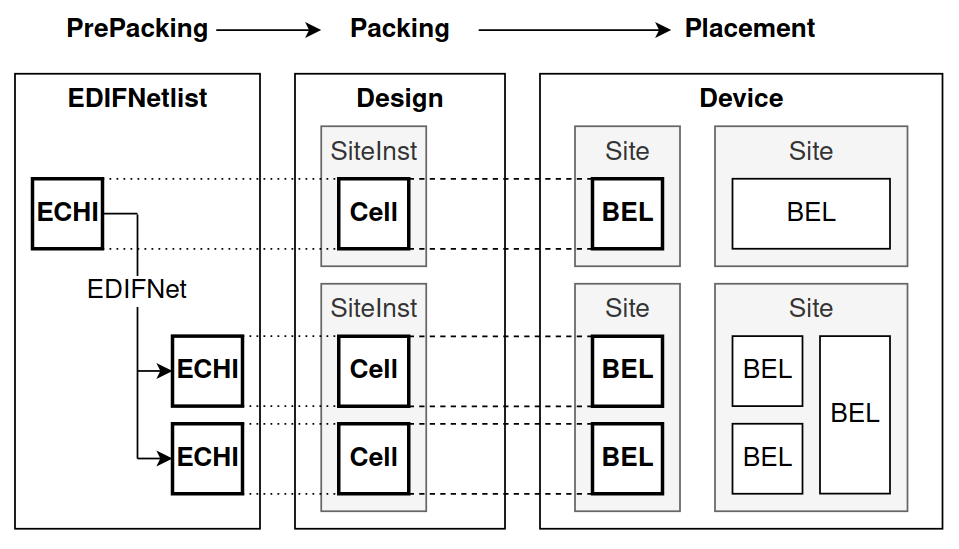
\includegraphics[width=0.9\columnwidth]{figures/edif_design_device.png}
    \captionof{figure}{Our placement workflow}
    \label{fig:edif_design_device}
}


\subsection{Prepacking}
\label{subsec:prepacking}


The first step in our placement flow is \textbf{prepacking}. 
Recall from the 7-Series architecture that there are certain multi-cell structures that must adhere to certain placements constraints to ensure legality, and by design, to minimize wirelength. 
The job of the prepacker is to traverse the raw EDIF netlist, detect these multi-cell structures, and consolidate these cells into clusters or groups of clusters that naturally reflect these placement constraints. 

Recall that \texttt{CARRY4} chains must necessarily be placed vertically and consecutively across a column of SLICEs in ascending order. 
Likewise, \texttt{DSP48E1} cascades must necessarily be placed vertically and consecutively across a column of \texttt{DSP48E1} Sites in ascending order. 
A LUT-FF pair may be placed freely, but should be placed in the same lane within the same SLICE to minimize wirelength.

The raw EDIF netlist only tells us the list of nets and the cell ports that they connect to. 
It does not report the presence of any multi-cell structures (\texttt{CARRY4} chains, etc.). 
Thus, we must traverse the netlist to detect these multi-cell structures and store that structure information in a class we will call \texttt{PrepackedDesign}.

The code snippet in \ref{lst:carry_chains} shows how one can detect and collect these \texttt{CARRY4} chains using RapidWright. 
We first collect the cells in the design that are of type \texttt{CARRY4}, then iteratively traverse their Carry-Out (\texttt{CO}) to Carry-In (\texttt{CI}) nets to find incident \texttt{CARRY4} cells.
Each \texttt{CARRY4} chain has an anchor cell and a tail cell where the chain terminates.
The anchor is found when the \texttt{CI} net connects to Ground (\texttt{GND}), while the tail is found when the \texttt{CO} port is null. 
We can further detect if there are \texttt{LUT}s or \texttt{FF}s connected to the \texttt{CARRY4} cell and store that information in a data structure we will call \texttt{CarryCellGroup} as defined in figure \ref{fig:substages}.
This will help us in knowing which cells can be packed together into the same \texttt{Site} in the subsequent stages. 

Similarly, \texttt{DSP48E1} cascades can be found and collected by traversing the \texttt{PCOUT} \texttt{ACOUT} and \texttt{BCOUT} nets.
\texttt{LUT-FF} pairs can be found by inspecting the LUT output (O) net and checking for FF input (DI) ports. 
We can bucket these LUT-FF pairs by finding the set of unique \texttt{CE} \texttt{SR} net pairs to know which group of LUT-FF pairs can be placed within the same \texttt{Site}. 

We detect the presence of these multi-cellular structures and consolidate that information into our \texttt{PrepackedDesign} object in preparation for the following Packing stage. 


\end{multicols}
{
    \centering
    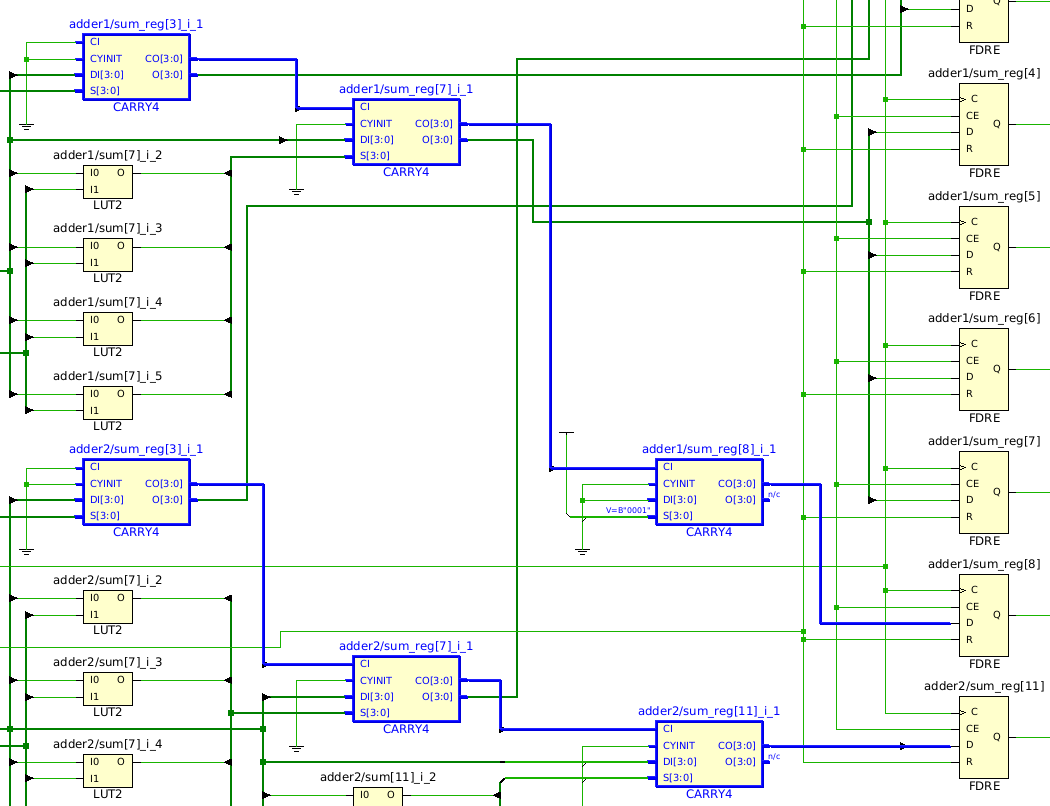
\includegraphics[width=0.8\columnwidth]{figures/carry_chain_traversal.png}
    \captionof{figure}{A netlist with two \texttt{CARRY4} chains, each of size 3}
    \label{fig:carry_chain_traversal}
}
\begin{multicols}{2}


\begin{lstlisting}[caption={Code Printout}]
Anchor Cell: adder2/sum_reg[3]_i_1, CellType: CARRY4
	Cell: adder2/sum_reg[7]_i_1, CellType: CARRY4
	Cell: adder2/sum_reg[11]_i_1, CellType: CARRY4
Anchor Cell: adder1/sum_reg[3]_i_1, CellType: CARRY4
	Cell: adder1/sum_reg[7]_i_1, CellType: CARRY4
	Cell: adder1/sum_reg[8]_i_1, CellType: CARRY4
\end{lstlisting}


\begin{lstlisting}[language=java, caption={Finding and storing carry chains.}, label={lst:carry_chains}]
Design design = Design.readCheckpoint("synth.dcp")
EDIFNetlist netlist = design.getNetlist();
List<EDIFCellInst> ecis = netlist.getAllLeafCellInstances();

// Select only the carry cells.
List<EDIFCellInst> carryCells = new ArrayList<>();
for (EDIFCellInst eci : ecis) {
    if (eci.getCellName().equals("CARRY4"))
        carryCells.add(eci);
}

// Find and remove carry chains until the list is empty
List<List<EDIFCellInst>> carryChains = new ArrayList<>();
while (!carryCells.isEmpty()) {
    // Arbitrarily set "currentCell" pointer to a cell in the list
    EDIFCellInst currentCell = carryCells.get(0);

    // Find this carry chain anchor.
    // Traverse the Carry-In (CI) to Carry-Out (CO) nets.
    // Anchor is found when net on the CI Port is Ground.
    while (true) {
        System.out.println(currentCell);
        // Access the CI port on this cell.
        EDIFPortInst sinkPort = currentCell.getPortInst("CI");
        // Access the net on this CI port.
        EDIFNet net = sinkPort.getNet();
        if (net.isGND()) {
            // Found this chain anchor!
            break;
        }
        // Get all ports on this net.
        List<EDIFPortInst> netPorts = net.getPortInsts();
        for (EDIFPortInst netPort : netPorts) {
            // Access the port belonging to another carry cell.
            EDIFCellInst sourceCell = netPort.getCellInst();
            if (sourceCell.getCellName().equals("CARRY4")) {
                // Move the "currentCell" pointer
                currentCell = sourceCell;
                break;
            }
        }
    }



    // Now we have the chain anchor as currentCell.
    // Now traverse in the opposite direction to find the chain tail.
    // Tail is found when the CO Port is null.
    // Collect the chain cells into an ordred list.
    List<EDIFCellInst> currentChain = new ArrayList<>();
    currentChain.add(currentCell);
    while (true) {
        EDIFPortInst sourcePort = currentCell.getPortInst("CO[3]");
        if (sourcePort == null) {
            // Found this chain's tail!
            break;
        }
        EDIFNet net = sourcePort.getNet();
        List<EDIFPortInst> netPorts = net.getPortInsts();
        for (EDIFPortInst netPort : netPorts) {
            EDIFCellInst sinkCell = netPort.getCellInst();
            if (netPort.getName().equals("CI") &&
                    sinkCell.getCellName().equals("CARRY4")) {
                currentCell = sinkCell;
                // Add the cell to the chain list.
                currentChain.add(currentCell);
                break;
            }
        }
    }
    // Add currentChain to the list of chains
    carryChains.add(currentChain);
    // Remove currentChain from the list of cells
    carryCells.removeAll(currentChain);
} // end while()

// Print out the carry chains. 
for (List<EDIFCellInst> chain : chains) {
    for (int i = 0; i < chain.size(); i++) {
        EDIFCellInst carry = chain.get(i);
        if (i == 0) {
            writer.write("\nAnchor Cell: " + carry.getName() + 
                ", CellType: " + carry.getCellName());
        } else {
            writer.write("\n\tCell: " + carry.getName() + 
                ", CellType: " + carry.getCellName());
        }
    }
}
\end{lstlisting}
\newpage




\subsection{Packing}
\label{subsec:packing}
Now that we have our \texttt{PrepackedDesign} object keeping track of multi-cell structures on the \texttt{edif} level, we can start packing them into \texttt{SiteInst} objects on the \texttt{design} level. 
Below are some of the most relevant classes from the \texttt{design} package for this task.
\begin{itemize}
    \item \texttt{Cell}: A cell corresponds to the leaf cell within the logical netlist \texttt{EDIFCellInst} and provides a mapping to a physical location BEL on the device. A cell can be created directly out of an \texttt{EDIFCellInst} to inherit all of its \texttt{edif} properties on the \texttt{design} level.
    \item \texttt{Net}: Represents the physical net to be routed (both inter-site and intra-site). When an \texttt{Cell} is created out of an \texttt{EDIFCellInst}, the \texttt{Net}s are automatically created out of its corresponding \texttt{EDIFNet}s.
    \item \texttt{SiteInst}: An instance of a \texttt{Site} on the \texttt{Device}. Carries the mapping information between the \texttt{BEL}s in a \texttt{Site} and the \texttt{Cell}s assigned to them. Also keeps track of the intra-Site routing information within (\texttt{Net}s, \texttt{SitePinInst}s, \texttt{SitePIP}s, etc.).
    \item \texttt{SitePIP}: A Programmable Interconnect Point (PIP) in a \texttt{Site}. Represents the fuses in intra-Site routing \texttt{BEL}s. 
    \item \texttt{SitePinInst}: An instance of a \texttt{SitePin} on a \texttt{Site}. These objects serve as the interface between intra-Site routing and general inter-Site routing. 
\end{itemize}
\columnbreak


A new \texttt{SiteInst} is created by populating its BELs with existing \texttt{EDIFHierCellInst} objects from the \texttt{EDIFNetlist}, and is immediately placed on a specific \texttt{Site}. 
The packer therefore assigns an initial placement to every \texttt{SiteInst} before the simulated‐annealing stage randomizes their positions. 
During this packing phase, we simply pseudorandomly map \texttt{design} \texttt{SiteInst}s onto \texttt{device} \texttt{Site}s in coordinate order as they are generated (e.g., the first \texttt{SiteInst} onto \texttt{SLICEL\_X0Y0}, the second onto \texttt{SLICEL\_X0Y1}, and so on). 

One can think of a \texttt{design} \texttt{SiteInst} as a movable square peg and the corresponding \texttt{device} \texttt{Site} as a fixed square hole. 
Both \texttt{SiteInst}s and \texttt{Site}s come in various shapes or types (\texttt{SLICEL}, \texttt{SLICEM}, \texttt{DSP48E1}, etc.) and placement is only allowed between compatible pairs. 
For example, a \texttt{RAMB48E1} \texttt{SiteInst} can only be placed on a \texttt{RAMB48E1} \texttt{Site}.
A \texttt{DSP48E1} \texttt{SiteInst} can only be placed on a \texttt{DSP48E1} \texttt{Site}.
A \texttt{SLICEL} \texttt{SiteInst} may occupy either a \texttt{SLICEL} or a \texttt{SLICEM} \texttt{Site}, whereas a \texttt{SLICEM} \texttt{SiteInst} can only be placed on a \texttt{SLICEM} \texttt{Site}.
These constraints must be followed as the \texttt{SiteInst}s move across the device throughout the placement stage to ensure legality. 


\end{multicols}
\begin{lstlisting}[caption=\texttt{SiteInst} constructor and methods.]
SiteInst Constructor: 
    SiteInst(String name, Design design, SiteTypeEnum type, Site site)

Most relevant SiteInst Methods:
    createCell(EDIFHierCellInst inst, BEL bel) // Populating the SiteInst BELs with Cells
    unplace() // Unplacing the SiteInst from its current Site
    place(Site site) // Placing an unplaced SiteInst onto a Site
    routeSite() // Attempt to automatically route all intra-Site nets (manual intervention likely required)
    routeIntraSiteNet(Net net, BELPin src, BELPin snk) // Manually route an intra-Site net

Example:
    SiteInst si = new SiteInst("mySiteInst", design, SiteTypeEnum.SLICEL, device.getSite("SLICEL_X0Y1"));
    si.createCell(someFDRECell, si.getBEL("AFF"));
    si.routeSite();
    si.unplace();
    si.place(device.getSite("SLICEL_X15Y33"));
    // In Simulated Annealing, SiteInst objects will be unplaced() and placed() many times to converge to an optimal solution. 
    // All Cell-BEL mapping and intra-Site routing is preserved when a SiteInst is moved. 

\end{lstlisting}


\begin{lstlisting}[language=java, caption={Packing an individual \texttt{CarryCellGroup} into one \texttt{SLICEL} \texttt{SiteInst}s.}, label={lst:single_carry_chains}]
protected String[] FF_BELS = new String[] { "AFF", "BFF", "CFF", "DFF" };
protected String[] LUT6_BELS = new String[] { "A6LUT", "B6LUT", "C6LUT", "D6LUT" };

private void packCarrySite(CarryCellGroup carryCellGroup, SiteInst si) {
    // potential bug: what guarantees that all of the FFs connected to the CARRY4 all share the same CE and Reset?
    for (int i = 0; i < 4; i++) {
        EDIFHierCellInst ff = carryCellGroup.ffs().get(i);
        if (ff != null)
            si.createCell(ff, si.getBEL(FF_BELS[i]));
        EDIFHierCellInst lut = carryCellGroup.luts().get(i);
        if (lut != null)
            si.createCell(lut, si.getBEL(LUT6_BELS[i]));
        // carry site LUTs MUST be placed on LUT6 BELs.
        // only LUT6/O6 can connect to CARRY4/S0
    }
    si.createCell(carryCellGroup.carry(), si.getBEL("CARRY4"));
    // default intrasite routing
    si.routeSite();
    // sometimes the default routeSite() is insufficient, so some manual
    // intervention is required
    rerouteCarryNets(si);
    rerouteFFClkSrCeNets(si);
} // end placeCarrySite()
\end{lstlisting}

\newpage
\begin{lstlisting}[language=java, caption={Packing \texttt{CarryCellGroup}s into \texttt{SLICEL} \texttt{SiteInst}s.}, label={lst:carry_chains}]
private List<List<SiteInst>> packCarryChains(List<List<CarryCellGroup>> EDIFCarryChains)
        throws IOException {
    List<List<SiteInst>> siteInstChains = new ArrayList<>();
    writer.write("\n\nPacking carry chains... (" + EDIFCarryChains.size() + ")");
    for (List<CarryCellGroup> edifChain : EDIFCarryChains) {
        List<SiteInst> siteInstChain = new ArrayList<>();
        writer.write("\n\t\tChain Size: (" + edifChain.size() + "), Chain Anchor: "
                + edifChain.get(0).carry().getFullHierarchicalInstName());
        Site anchorSite = selectCarryAnchorSite(edifChain.size());
        SiteTypeEnum selectedSiteType = anchorSite.getSiteTypeEnum();
        for (int i = 0; i < edifChain.size(); i++) {
            Site site = (i == 0) ? anchorSite
                    : device.getSite("SLICE_X" + anchorSite.getInstanceX() + "Y" + (anchorSite.getInstanceY() + i));
            SiteInst si = new SiteInst(edifChain.get(i).carry().getFullHierarchicalInstName(), design,
                    selectedSiteType,
                    site);
            packCarrySite(edifChain.get(i), si);
            if (i == 0) { // additional routing logic for anchor site
                Net CINNet = si.getNetFromSiteWire("CIN");
                CINNet.removePin(si.getSitePinInst("CIN"));
                si.addSitePIP(si.getSitePIP("PRECYINIT", "0"));
            }
            occupiedSites.get(selectedSiteType).add(site);
            availableSites.get(selectedSiteType).remove(site);
            siteInstChain.add(si);
        }
        siteInstChains.add(siteInstChain);
    } // end for (List<EDIFCellInst> chain : EDIFCarryChains)
    return siteInstChains;
} // end packCarryChains()

\end{lstlisting}


\begin{lstlisting}[language=java, caption={Manually rerouting intra-Site nets in a \texttt{SLICEL} containing \texttt{CARRY4}}]
    protected String[] FF_BELS = new String[] { "AFF", "BFF", "CFF", "DFF" };
    private void rerouteCarryNets(SiteInst si) {
        // activate PIPs for CARRY4/COUT
        si.addSitePIP(si.getSitePIP("COUTUSED", "0"));
        // undo default CARRY4/DI nets
        SitePinInst AX = si.getSitePinInst("AX");
        if (AX != null)
            si.unrouteIntraSiteNet(AX.getBELPin(), si.getBELPin("ACY0", "AX"));
        SitePinInst DX = si.getSitePinInst("DX");
        if (DX != null)
            si.unrouteIntraSiteNet(DX.getBELPin(), si.getBELPin("DCY0", "DX"));
        // activate PIPs for CARRY4/DI pins
        si.addSitePIP(si.getSitePIP("DCY0", "DX"));
        si.addSitePIP(si.getSitePIP("CCY0", "CX"));
        si.addSitePIP(si.getSitePIP("BCY0", "BX"));
        si.addSitePIP(si.getSitePIP("ACY0", "AX"));
        // remove stray CARRY4/CO nets
        if (si.getNetFromSiteWire("CARRY4_CO2") != null)
            design.removeNet(si.getNetFromSiteWire("CARRY4_CO2"));
        if (si.getNetFromSiteWire("CARRY4_CO1") != null)
            design.removeNet(si.getNetFromSiteWire("CARRY4_CO1"));
        if (si.getNetFromSiteWire("CARRY4_CO0") != null)
            design.removeNet(si.getNetFromSiteWire("CARRY4_CO0"));
        // add default XOR PIPs for unused FFs
        for (String FF : FF_BELS)
            if (si.getCell(FF) == null)
                si.addSitePIP(si.getSitePIP(FF.charAt(0) + "OUTMUX", "XOR"));
    } // end rerouteCarryNets()
\end{lstlisting}
\begin{multicols}{2}



\subsection{Placement}
    \label{subsec:placement}
    Up until now we have only organized the logical \texttt{EDIFHierCellInst}s into \texttt{SiteInst}s. 
    This is where simulated annealing actually begins where we actually place the \texttt{SiteInst}s onto physical \texttt{Site}s on the \texttt{device} level. 



\section{Placement}
\label{sec:placement}
So far we have only dealt with technology problems where we consider the problem space and adress the constraints of the hardware architecture. 
For every constraint, we devise a solution to fully address it or a simplification that sacrifices some optimization but reduces the complexity of the problem space. 

Now that we have dealt with the bulk of these constraints and squared them away into self-contained \texttt{SiteInst}s, we can now more easily apply some general optimization algorithms to finally address our optimization objective, which is to place these \texttt{SiteInst} objects onto the device while minimizing wirelength. 

\subsection{Simulated Annealing}
\label{subsec:simulated_annealing}

In this paper we implement and present a basic Simulated Annealing (SA) placer. 
As mentioned in the Introduction, SA is a metaheuristic that approximates a global optimum in a large optimization search space. 
SA does not guarantee a globally optimal solution, but provides solutions that are often "good enough", especially when finding an approximate global optimum is more important than finding a precise local optimum in a fixed amount of time. 
SA is typically employed in discrete combinatorial optimization problems like the travelling salesman problem or job-shop scheduling. 
It is directly inspired by Annealing in metallurgy, which is the physical process of heating a metal above its crystallization temperature, allowing its atoms to migrate through the crystal lattice, and slowly cooling it to allow its atoms to recrystallize into a more desirable structure, such as one that minimizes structural defects. 

The state \(s\) of the system and the function \(E(s)\) to be minimized is analogous to the internal energy of the system. 
In metallurgic Annealing, the state \(s\) represents the position of every atom in the metal object at any given snapshot in time, while \(E(s)\) represents the defectiveness in the metal's structure however that may be quantified. 
In the context of our SA placer, the state \(s\) represents the placement of every \texttt{SiteInst} on the \texttt{device} at any given iteration, while \(E(s)\) represents the total wirelength of \texttt{Net}s between all \texttt{SiteInst}s of the current placement.
We will be measuring wirelength using the manhattan distance between the 2-dimensional coordinates of the \texttt{SiteInst}s on the \texttt{device}.
We will refer to these distances as half perimeter wirelength (HPWL).
The goal of SA is to bring the system from some initial state to a state with lower energy until some stopping criterion is met, whether that be when a computational budget is exceeded, an energy budget is met, or until the energy's rate of change approaches zero. 

At each step or iteration, the algorithm considers some neighboring state \(s^*\). 
If \(s^*\) has a lower energy than \(s\), then the state transition from \(s\) to \(s^*\) is accepted outright.
If \(s^*\) has a higher energy, then it can probabilistically be accepted depending on the current global temperature.
The higher the temperature, the higher the likelihood of accepting an energy-increasing move. 
The global temperature starts at some positive amount then gradually decreases to zero according to a cooling schedule.
This cooling schedule can be linear, geometric, logarithmic, or some piecewise combination. 
Its parameters can be fine tuned through empirical experimentation. 

Shown in Listing \ref{lst:sa_outer} is a simplified pseudocode for the outer-most loop of our placer's SA algorithm. 
First, we randomly place all \texttt{SiteInst}s across the \texttt{device}.
Then, we initialize a simple geometric cooling schedule: 
\begin{equation}
    \label{coolingSchedule}
    T_{n+1} = \alpha T_n
\end{equation}
with initial temperature \(T_0=10000\), cooling rate \(\alpha=0.98\), and \(n = \{0, 1, 2, ..., 300\}\) passes.
Hill-climbing moves can be accepted via the probability function \(P()\): 
\begin{equation}
    \label{moveAcceptance}
    P(s, s^*, T_n) = exp(\frac{E(s) - E(s^*)}{T_n})
\end{equation}
where \(E(s^*)\) is the energy of the proposed state \(s^*\), \(E(s)\) is the energy of the current state \(s\), and \(T_n\) is the current global temperature at \(n\) passes. 
If \(P(s, s^*, T_n) < random(0, 1)\), then \(s \leftarrow s^*\).
Recall that this probability is only evaluated for hill-climbing moves, thus the cost difference \(E(s) - E(s^*)\) is always negative.
In summary, a lower the cost difference and a higher the temperature contributes to a higher the probabilty of hill-climbing acceptance.
All hill-descending moves on the other hand are simply accepted outright. 

Then, we enter the outer-most loop which terminates when the number of passes exceeds our computational budget, in this case, 300 passes. 
In each pass, we \texttt{moveAll()} the design, then update the global temperature. 

In each \texttt{moveAll()}, we iterate through four mutually exclusive groups of placement objects: \texttt{DSPSiteInstCascades}, \texttt{CARRYSiteInstChains}, \texttt{RAMSiteInst}s, and \texttt{CLBSiteInst}s (single SLICEs that do not belong to CARRY chains).
For each placement object in the pass, we propose a new placement for that object on the device. 
Each proposed movement represents a proposed state transition of system. 
If the design has for example, 50 \texttt{DSPSiteInstCascades}, 100 \texttt{CARRYSiteInstChains}, 75 \texttt{RAMSiteInst}s, and 250 \texttt{CLBSiteInst}s, and we set a budget of 300 passses, then the algorithm will consider up to \(300 * (50 + 100 + 75 + 250) = 142500\) state transitions. 
If the proposed \texttt{Site} is already occupied by a resident or existing \texttt{SiteInst}, we evaluate a swap in their placements. 

In SA, proposed movements are selected randomly, then accepted or rejected based on legality and cost. 
Figure \ref{fig:swapSingleSite} shows how a swap proposal between singular \texttt{CLBSiteInst}s or between \texttt{RAMSiteInst}s is evaluated, while Listing \ref{lst:sa_move_single} shows the corresponding Java code.
On the other hand, the movement of \texttt{SiteInst} chains is considerably more complex because there are more placement constraints to consider, especially when swapping the positions between multiple chains.
Figure \ref{fig:swapSiteChain} shows a demonstration of how two \texttt{DSPSiteInstCascades} or two \texttt{CARRYSiteInstChains} can be swapped while Listing \ref{lst:chain_swap_pseudocode} shows the corresponding pseudocode. 

In more sophisticated placers, the proposed movement can also be selected by finding the centroid between \texttt{SiteInst}s that share a net with the current object, or even a hybrid of random and centroid selection. 
Moves that actively attempt to predict a better placement are often referred to as "directed" moves in literature. 
Placers that take inspiration from physical interactions like gravity or electrostatics are often referred to as "force directed" moves and are akin to physics simulators. 

Directed moves as opposed to undirected moves give rise to the concept of legalization. 
When using undirected moves as in SA, we can simply keep track of a \texttt{List} or \texttt{HashMap} of occupied \texttt{Site}s and available \texttt{Site}s and select from that data structure via random selection. 
However, for directed moves like centroid selection, the centroid between \texttt{Site}s may not necessarily fall directly on another discrete \texttt{Site} on the \texttt{device}. 
Even when it does, the centroid \texttt{Site} may be incompatible with the \texttt{SiteInst} or may fail to meet some other placement constraint. 
In such cases, we must do a neighborhood search around the centroid up to a certain radius to find a \texttt{Site} that satisfies all the constraints of the \texttt{SiteInst} at hand. 
We will take some inspiration from ray-marching in graphics and do a diamond-shaped spiral search around the centroid where we check the legality of each \texttt{Site} as we step through the spiral and select the first \texttt{Site} that meets all of the placement constraints. 

In force directed moves, there is a concept of global placement versus detailed placement, where global placement is driven by forces and detailed placement attempts to legalize the global placement by discretizing it onto the grid of \texttt{Site}s on the device.
There also exists other strategies to mix packing, placement, and legalization in different ways. (CITE THAT ONE PAPER).
In this context, our placer follows a straightforward pack-legalize-place strategy. 

If the move reduces the HPWL cost, then the movement is accepted outright.
If the move increases cost, then it can be accepted by chance if the global temperature is high enough to permit the hill-climb.
The temperature decreases with each pass until reaching zero, at which point, the algorithm makes exclusively energy-decreasing moves, effectively reducing into a greedy algorithm. 
The hope is that by this point, the placement has already crystallized into an approximate global optimum and the greediness of the algorithm will help the system settle deeper into the energy well faster. 
We can also switch from random selection to centroid selection when the temperature approaches near zero to speed up the convergence further. 



\newcolumn
\begin{lstlisting}[language=java, caption={SA pseudocode: outer loop}, label={lst:sa_outer}]
public void placeDesign(PackedDesign packedDesign) {
    randomInitialPlacement(packedDesign);
    // init_temp=10000, alpha=0.98, max_passes=300
    initCoolingSchedule(10000, 0.98, 300)
    int passes = 0;
    while (passes < 300) {
        updateTemperature(passes);
        moveAll(packedDesign)
        passes++;
    }
}

private void moveAll(PackedDesign packedDesign) {
    moveSiteChains(packedDesign.DSPSiteInstCascades);
    moveSiteChains(packedDesign.CARRYSiteInstChains);
    moveSingleSite(packedDesign.RAMSiteInsts);
    moveSingleSite(packedDesign.CLBSiteInsts);
}
\end{lstlisting}


\begin{lstlisting}[language=java, caption={Single Site Movement}, label={lst:sa_move_single}]
protected void moveSingleSite(List<SiteInst> sites) {
for (SiteInst si : sites) {
    SiteTypeEnum ste = si.getSiteTypeEnum();
    List<Site> homeConns = findConnectedSites(si, null);
    Site homeSite = si.getSite();
    Site awaySite = proposeSite(si, homeConns, true);
    SiteInst awaySi = occupiedSites.get(ste).get(awaySite);
    double oldCost = 0;
    double newCost = 0;
    if (awaySi != null) {
        List<Site> awayConns = findConnectedSites(awaySi, null);
        oldCost += evaluateSite(homeConns, homeSite);
        oldCost += evaluateSite(awayConns, awaySite);
        newCost += evaluateSite(homeConns, awaySite);
        newCost += evaluateSite(awayConns, homeSite);
    } else {
        oldCost += evaluateSite(homeConns, homeSite);
        newCost += evaluateSite(homeConns, awaySite);
    }
    if (evaluateMoveAcceptance(oldCost, newCost)) {
        if (awaySi != null) {
            unplaceSiteInst(si);
            unplaceSiteInst(awaySi);
            placeSiteInst(si, awaySite);
            placeSiteInst(awaySi, homeSite);
        } else {
            unplaceSiteInst(si);
            placeSiteInst(si, awaySite);
        }
    }
}
} // end randomMoveSingleSite()
\end{lstlisting}

{
    \centering
    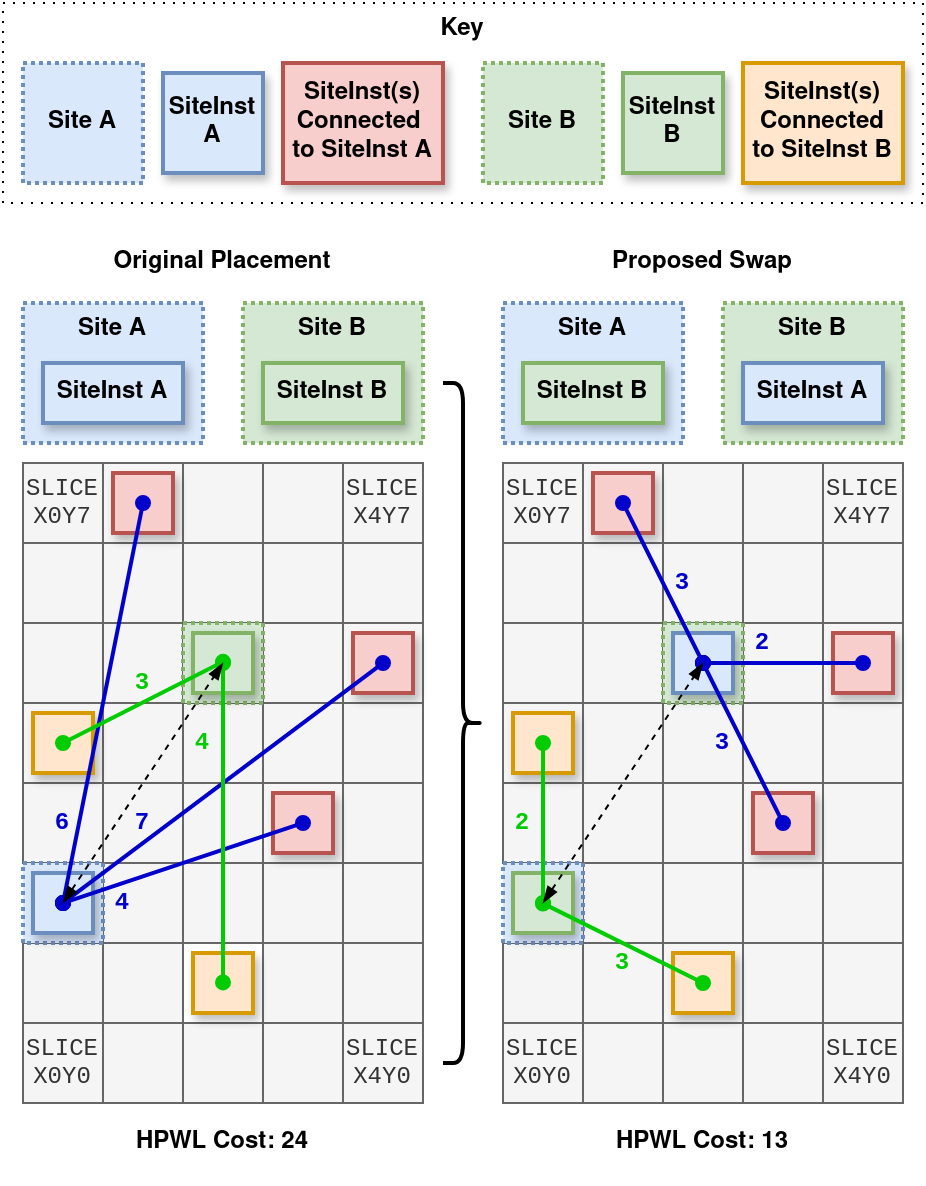
\includegraphics[width=\columnwidth]{figures/placement/swapSingleSite.png}
    \captionof{figure}{Single Site Swap Proposal}
    \label{fig:swapSingleSite}
}
\vfill

\begin{lstlisting}[language=java, caption={Cooling Schedule and Move Acceptance with Temperature}, label={lst:sa_acceptance}]
protected List<Double> coolingSchedule;
public void initCoolingSchedule(double initialTemp, double alpha, int movesLimit) {
    double currentTemp = initialTemp;
    for (int i = 0; i < movesLimit; i++) {
        this.coolingSchedule.add(currentTemp);
        currentTemp *= alpha; // geometric cooling
    }
}

protected boolean evaluateMoveAcceptance(double oldCost, double newCost) {
    // if the new cost is lower, accept it outright
    if (newCost < oldCost)
        return true;
    // otherwise, evaluate probability to accept higher cost
    double delta = newCost - oldCost;
    double acceptanceProbability = 
        Math.exp(-delta / this.currentTemp);
    return Math.random() < acceptanceProbability;
}
\end{lstlisting}

\begin{lstlisting}[language=Java, caption={Chain Swapping Pseudocode}, label={lst:chain_swap_pseudocode}]
protected void moveSiteChains(List<List<SiteInst>> chains) {
for (List<SiteInst> currentChain : chains) {
    int chainSize = currentChain.size();

    // Step 1: Identify home window for this chain
    Site homeAnchor = currentChain.get(0).getSite();
    List<Site> homeWindow = getSitesInWindow(homeAnchor, chainSize);

    // Step 2: Select a candidate away anchor
    Site awayAnchor = proposeAnchorSite(currentChain, homeWindow, true);

    // Step 3: Determine away window based on awayAnchor and chainSize
    List<Site> awayWindow = getSitesInWindow(awayAnchor, chainSize);

    // Step 4: Find any resident SiteInst chains in the away window
    List<List<SiteInst>> residentChainsInAway = 
        collectChainsInWindow(siteType, awayWindow);

    // Step 5: If any resident chains overlap with the away window, extend the away window to fully accomodate them 
    if (!residentChainsInAway.isEmpty()) {
        awayWindow = extendWindowToIncludeChains(awayWindow, residentChainsInAway);
    }

    // Step 6: Map the (possibly extended) away window back onto the original region so that the tail of that window coincides with the tail of the current chain
    List<Site> candidateHomeWindow = mapAwayToHomeWindow(
        homeAnchor, awayWindow, chainSize);

    // Step 7: While the candidate home window still overlaps resident chains, shift upward
    int shifts = 0;
    while (windowHasOverlap(candidateHomeWindow)) {
        candidateHomeWindow = shiftWindowUp(candidateHomeWindow);
        shifts++;
        if (shifts > (homeWindow.size() - chainSize)) {
            // Reject this swap attempt.
            // Move on to the next chain.
            continue;
        }
    }

    // Step 8: Compute cost of the original placement in home window
    double oldCost = evaluateWindowCost(homeWindow);

    // Step 9: Compute cost of the proposed swap placement
    double newCost = evaluateWindowCostForSwap(
        homeWindow, awayWindow, currentChain);

    // Step 10: Decide whether to accept the move based on oldCost, newCost, and temperature
    if (evaluateMoveAcceptance(oldCost, newCost, currentTemp)) {
        // Step 11: Perform an element-wise swap of SiteInsts between homeWindow and awayWindow
        swapChainsBetweenWindows(homeWindow, awayWindow);
    }
}
}
\end{lstlisting}


\newpage
\end{multicols}
{
    \centering
    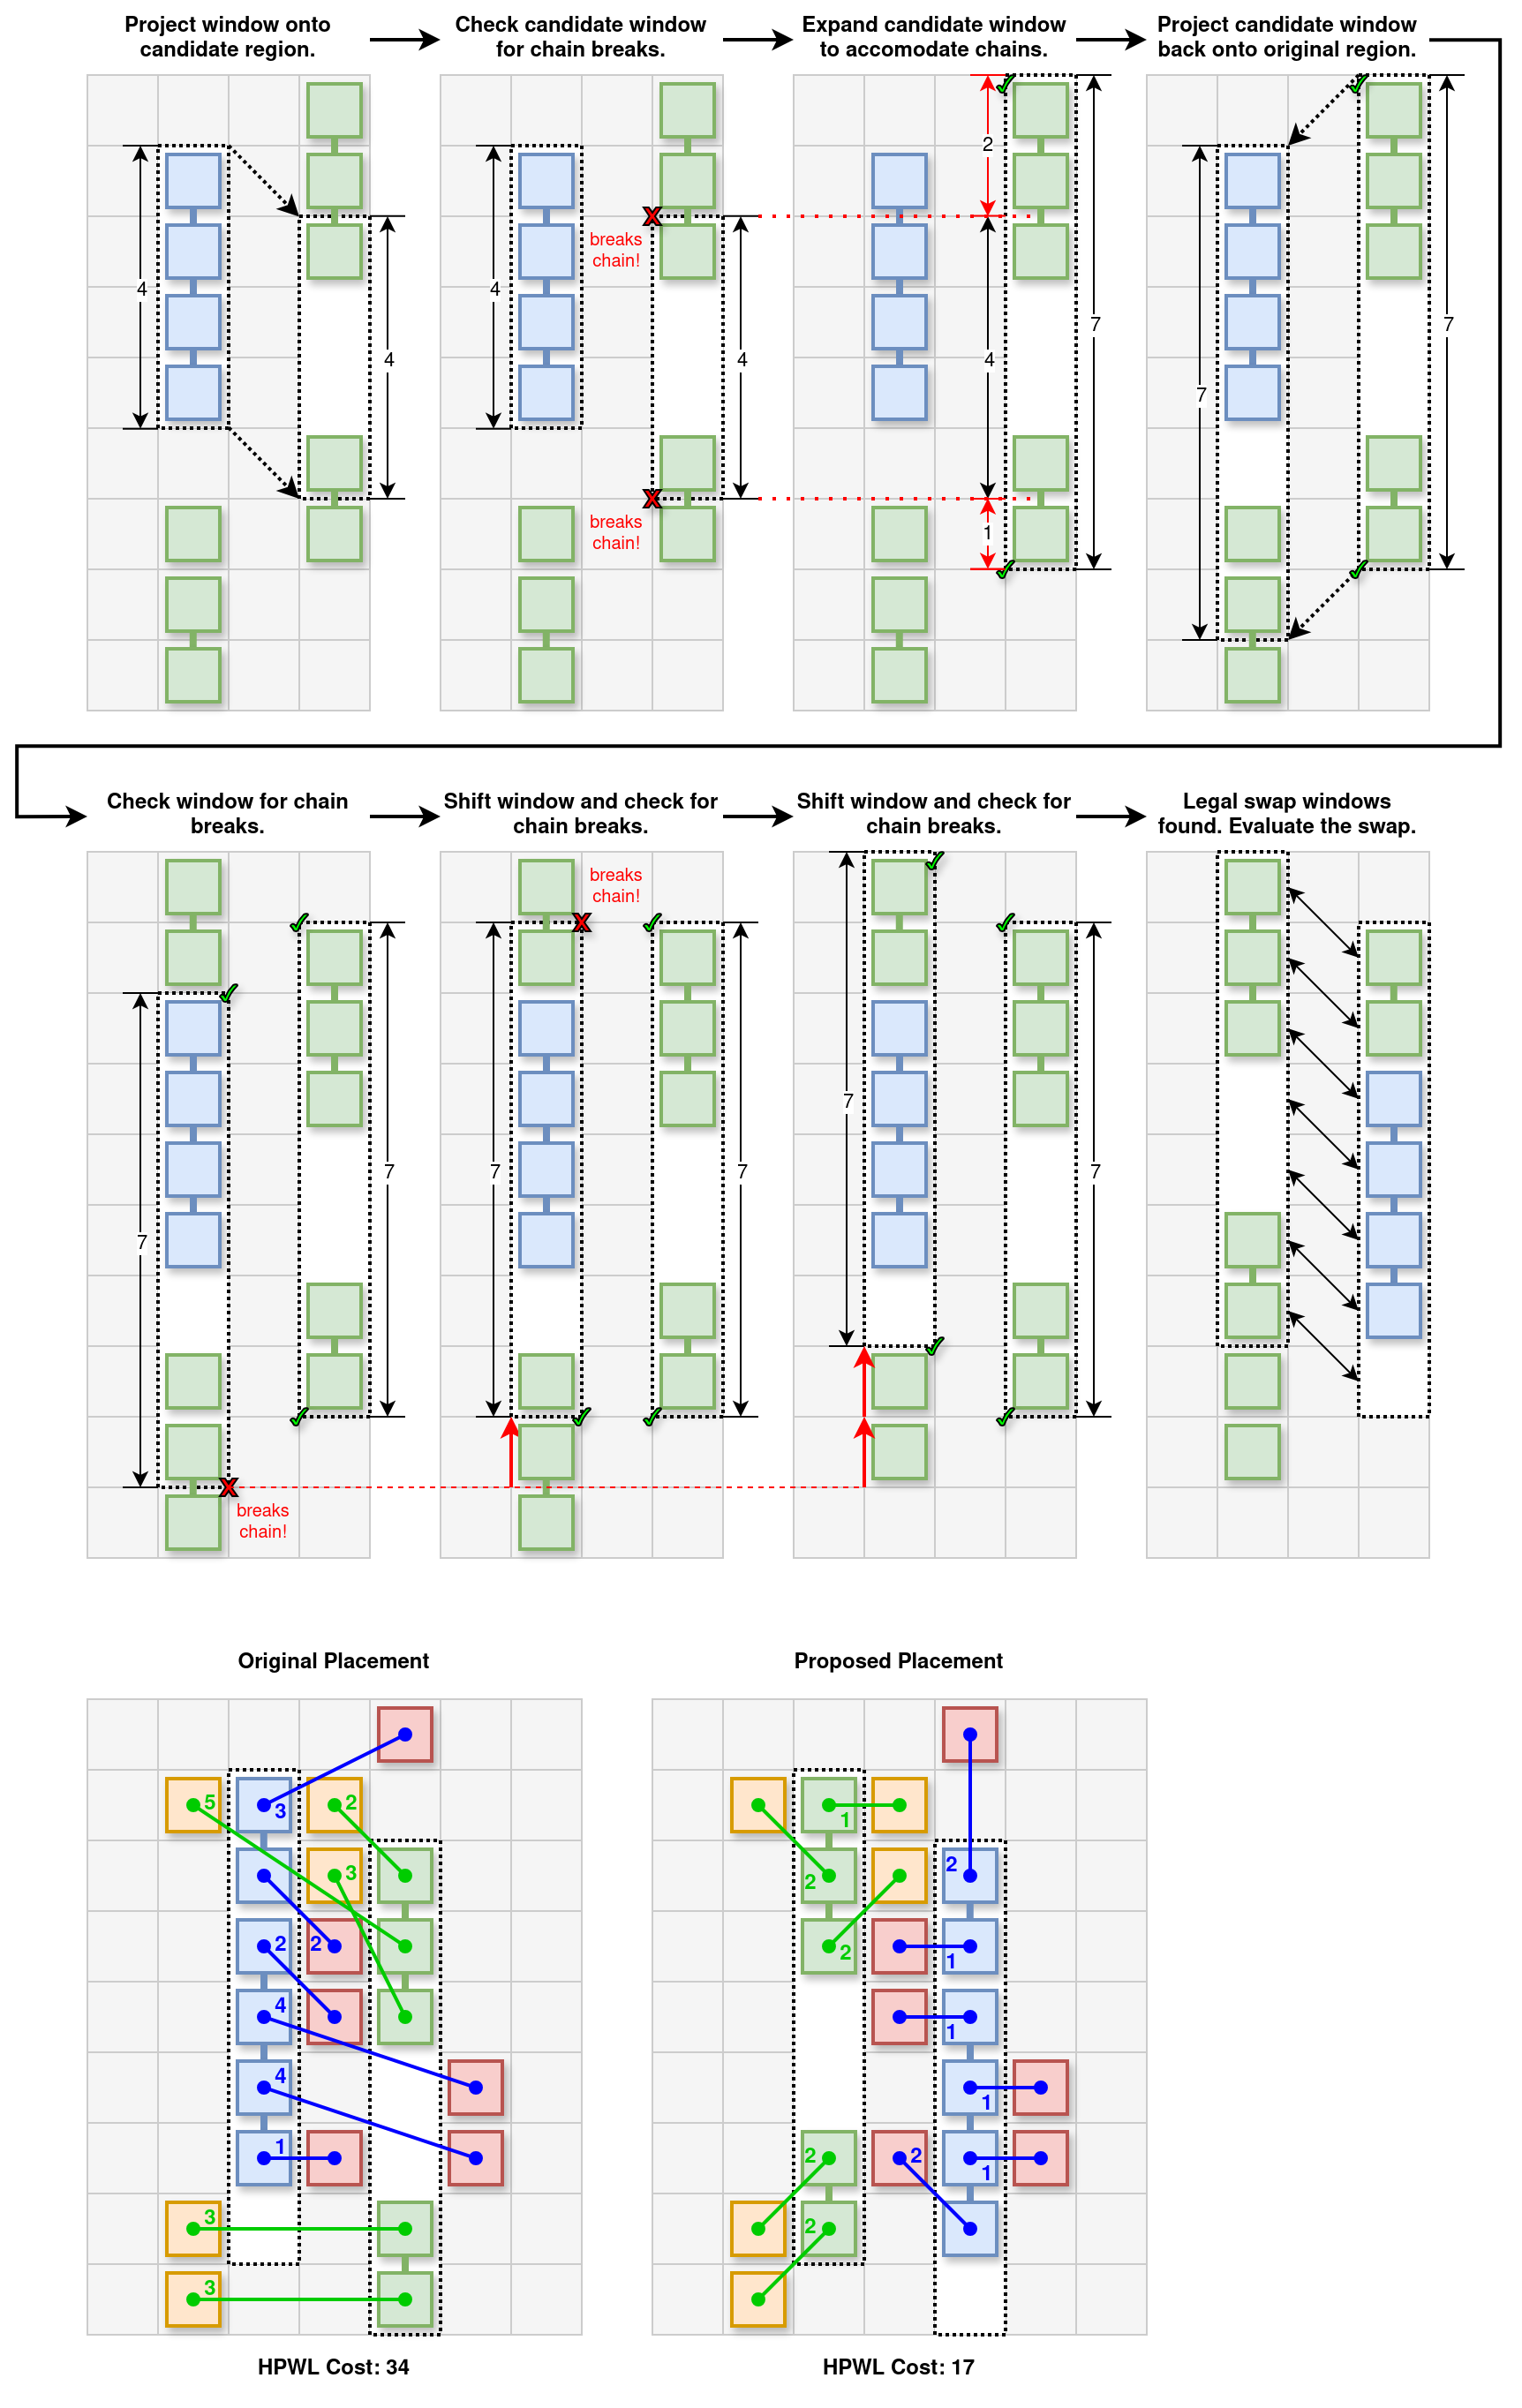
\includegraphics[width=0.9\columnwidth]{figures/placement/swapSiteChain.png}
    \captionof{figure}{Site Chain Swap Proposal}
    \label{fig:swapSiteChain}
}
\begin{multicols}{2}



\section{Placement Results}
\label{sec:results}


We will need an HDL design that utilizes a good mixture of LUTs, FFs, BRAMs, and DSPs at scale to demonstrate the robustness and performance of our placers. 
Any DSP subsystem can serve as a good candidate for such a demonstration. 
Here, we will perform placement on a 2048-order FIR Filter which was conveniently created as coursework for a VLSI course. 
After passing synthesis, the FIR Filter design calls for the primitive cells shown in the second column of table \ref{fig:utilization}.
We will perform placement of this design on a \texttt{xc7z020} FPGA, which is a mid-ranged Xilinx device containing the available BELs shown in the first column of table \ref{fig:utilization}.
Note that \texttt{LUT5-LUT6} pairs are counted as a single \texttt{LUT}.
% Also note that the number of \texttt{CARRY4} BELs is equal to the total number of \texttt{SLICEL} and \texttt{SLICEM} Sites combined and that the number of \texttt{LUT}s is equal to four times that amount while the number of \texttt{FF}s is equal to eight times that amount.

\vspace{0.25cm}
{
    \centering
    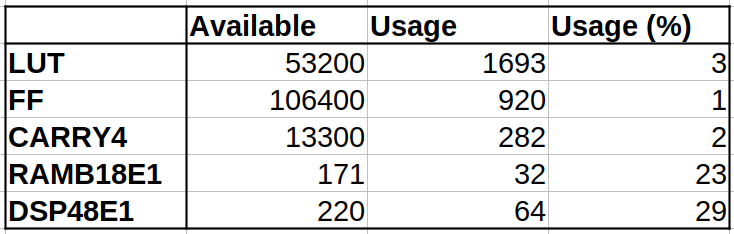
\includegraphics[width=0.8\columnwidth]{figures/results/utilization.png}
    \captionof{figure}{Utilization of BELs on a \texttt{xc7z020} FPGA for a FIR filter design}
    \label{fig:utilization}
}
\vspace{0.25cm}

Now, we present test results for a basic SA placer as well as test results for four simple variations as listed below. 
Note that midpoint simply means centroid.

\begin{itemize}
    \item \texttt{PlacerGreedyRandom}: all undirected random moves with greedy acceptance
    \item \texttt{PlacerGreedyMidpoint}: all directed centroid moves with greedy acceptance
    \item \texttt{PlacerAnnealRandom}: all undirected random moves with annealing acceptance \textbf{(the basic SA algorithm)}
    \item \texttt{PlacerAnnealMidpoint}: all directed centroid moves with annealing acceptance
    \item \texttt{PlacerAnnealHybrid}: \textbf{Initial:} 50\% random - 50\% centroid moves with annealing acceptance. \textbf{At Near-Zero Temperature:} 100\% centroid moves with annealing acceptance.
\end{itemize}

Shown in figure \ref{fig:placers_overlay} are the total HPWL curves over number of passes for each of the five placers. 
\texttt{PlacerGreedyMidpoint} (in red) appears to perform the worst by a considerable margin with a final HPWL cost of 590K.
This is likely due to the lack of randomness or lack of diversity in move proposals combined with the persistent greediness of the movement acceptance that prevents the system from escaping local minima.
This conclusion is supported by its HPWL curve (in red) showing a sharp drop in cost that quickly asymptotes just below the 600K mark, suggesting that the system crystallized very quickly into a local minimum and was unable to climb out of it.

Next is \texttt{PlacerAnnealMidpoint} with a final cost of 466K.
Like the previous placer, \texttt{PlacerAnnealMidpoint} lacks the diversity of random moves which contributes to faster crystallization into local minima.
However, this placer likely performed better than the previous as there is still some randomness in the move acceptance evaluation which gives way to occasional hill-climbing. 
Keep in mind that centroid moves do not necessarily decrease system cost. 
The centroid move can decrease the HPWL cost of the nets on connected to the current \texttt{SiteInst}, but can potentially increase the cost of another group of nets in the event of a swap, which can potentially result in an increase in total system cost.

The next three placers performed better than the previous two placers by decent margin.
The vanilla SA placer, \texttt{PlacerAnnealRandom}, is represented by the green curve.
We can observe that the cost decreases more steadily than the previous two placers, with noticeable spikes in total system cost due to hill-climbing, until settling at the 346K mark as the global temperature cools to zero.

Next is \texttt{PlacerGreedyRandom} which is represented by the purple curve.
We can observe a much steeper initial drop in system cost than the vanilla SA placer due to greedy movement acceptance.
Interestingly, this placer also settled at a lower final system cost of 333K, which is a slight 4\% improvement over vanilla SA.
We originally expected the greediness to be a detriment to finding the global minimum, but due to the inherent randomness of the algorithm, these broader trends will require many more test trials to reliably observe.

{
    \centering
    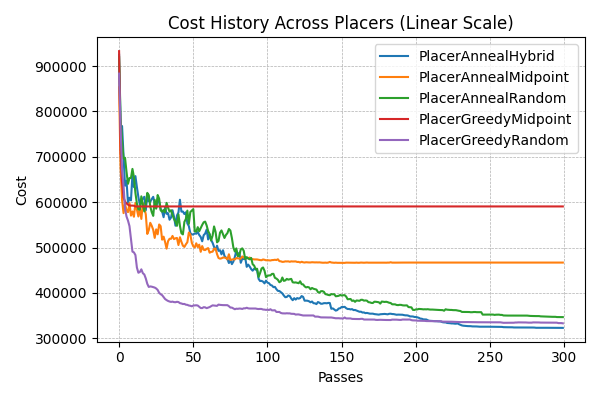
\includegraphics[width=\columnwidth]{figures/results/combined_cost_history_linear.png}
    \captionof{figure}{All placers overlaid}
    \label{fig:placers_overlay}
}

The best performing placer was \texttt{PlacerAnnealHybrid}, represented by the blue curve.
Starting at zero passes, the placer randomly selects between random selection and centroid selection, allowing the placer to make on average more cost-reducing moves, while still maintaining some diversity of moves for hill-climbing. 
Then, at near-zero temperature, the placer makes exclusively centroid moves with annealing acceptance to speed up the final crystallization into the local minimum. 
With centroid moves and annealing acceptance, hill-climbing can only be achieved via swaps.
We can observe that \texttt{AnnealHybrid} settles at a similar rate with the vanilla \texttt{AnnealRandom}, but eventually settles at a lower minimum at 322K, slightly outperforming \texttt{GreedyRandom}. 

{
    \centering
    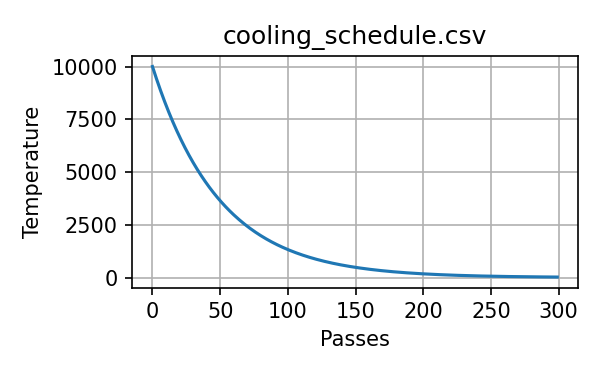
\includegraphics[width=0.6\columnwidth]{figures/placement/cooling_schedule_10000_98.png}
    \captionof{figure}{Cooling Schedule: \(T_0=10000\), \(\alpha=0.98\)}
    \label{fig:cooling_schedule_10000_98}
}

\newpage
Figures \ref{fig:PGRSnapshots}, \ref{fig:PGMSnapshots}, \ref{fig:PARSnapshots}, \ref{fig:PAMSnapshots}, and \ref{fig:PAHSnapshots} show snapshots of the placement progress on the physical \texttt{device} after 0, 10, 100, and 300 passes for each placer variant.

Please zoom into the document to render the figures in greater detail.
All black areas represent purely routing \texttt{Site}s that contain no logic resources. 
All gray or dull-colored boxes represent \texttt{Site}s that are unoccupied by \texttt{SiteInst}s, while brightly filled boxes represent \texttt{Site}s that are occupied by the supported library of \texttt{SiteInst}s.
Cyan boxes represent occupied \texttt{SLICEL}s, magenta boxes represent occupied \texttt{RAMB18E1}s, and yellow boxes represent occupied \texttt{DSP48E1}s.

The tangle of red lines represent the nets between the \texttt{Site}s, which are yet to be routed at this stage. 
Brighter red lines represent nets of higher total HPWL, while duller red lines represent nets of lower total HPWL.

Notice there are two brightly red nets in every figure that have a particularly high fan-out:
one sourced from the near-center, and another sourced from the top right of the device. 

The singular white box in the near-center of all of the figures represents an occupied \texttt{BUFGCTRL} \texttt{Site}, which is a clock buffer used to route clock trees. 
Since clock nets tend to have very high fanout, they can use up a significant portion of the routing resources if they are routed through general routing.
Modern FPGAs like the 7-Series have dedicated clock routes which can efficiently distribute clock signals to all logical \texttt{Site}s without burdening the general routing resources.
These special clock routes are accessed by routing the raw clock signal from the crystal oscillator IO port to one these on-chip clock buffers which connects to the on-chip clock tree network.
It is always best practice to use them to improve the routability of the design, and simultaneously, to reduce clock skew and improve timing. 
Our simple FIR Filter design only operates on a single clock domain, so only one clock buffer \texttt{Site} is used. 
An HDL design operating on many clock domains will use more clock buffers or a dedicated clock generator such as a phase locked loop (PLL) or mixed-mode clock manager (MCMM).

The right and left edges of the FPGA device is where most of the general purpose I/O (GPIO) is located. 
In the top right of the device is where we source our reset signal. 
Like the clock net, the reset net also has high fanout and is supplied to all synchronous elements.
Unlike clock signals, reset signals are not subject to sensitive timing constraints as they are not active on most clock cycles and can tolerate higher skew.
Thus, they are simply routed via general routing.

Observe how \texttt{PlacerGreedyMidpoint} \ref{fig:PGMSnapshots} and \texttt{PlacerAnnealMidpoint} \ref{fig:PAMSnapshots} both show almost not shrinkage in profile after the first 10 iterations, likely owing to the inability to hill-climb, while the other three placers show incremental shrinkage.

Also note the sparsity of the \texttt{DSP48E1} (yellow) and \texttt{RAMB18E1} (magenta) \texttt{Site} columns compared to the more uniform grid of \texttt{SLICEL}s (cyan).

\newpage
\end{multicols}
{
    \centering
    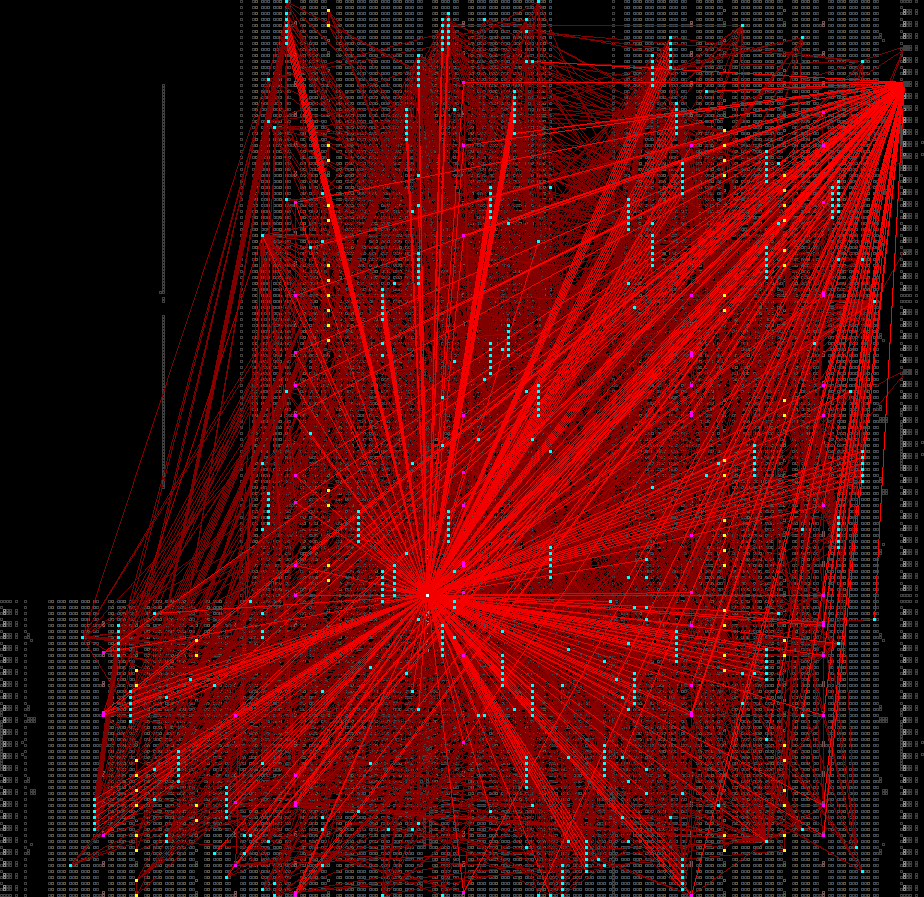
\includegraphics[valign=t, scale=0.13]{figures/results/PlacerGreedyRandom/random_placement.png}
    \includegraphics[valign=t, scale=0.13]{figures/results/PlacerGreedyRandom/00000010.png}
    \includegraphics[valign=t, scale=0.13]{figures/results/PlacerGreedyRandom/00000100.png}
    \includegraphics[valign=t, scale=0.13]{figures/results/PlacerGreedyRandom/00000299.png}
    \captionof{figure}{\texttt{PlacerGreedyRandom}}
    \label{fig:PGRSnapshots}
}

{
    \centering
    \includegraphics[valign=t, scale=0.13]{figures/results/PlacerGreedyMidpoint/random_placement.png}
    \includegraphics[valign=t, scale=0.13]{figures/results/PlacerGreedyMidpoint/00000010.png}
    \includegraphics[valign=t, scale=0.13]{figures/results/PlacerGreedyMidpoint/00000100.png}
    \includegraphics[valign=t, scale=0.13]{figures/results/PlacerGreedyMidpoint/00000299.png}
    \captionof{figure}{\texttt{PlacerGreedyMidpoint}}
    \label{fig:PGMSnapshots}
}

{
    \centering
    \includegraphics[valign=t, scale=0.13]{figures/results/PlacerAnnealRandom/random_placement.png}
    \includegraphics[valign=t, scale=0.13]{figures/results/PlacerAnnealRandom/00000010.png}
    \includegraphics[valign=t, scale=0.13]{figures/results/PlacerAnnealRandom/00000100.png}
    \includegraphics[valign=t, scale=0.13]{figures/results/PlacerAnnealRandom/00000299.png}
    \captionof{figure}{\texttt{PlacerAnnealRandom}}
    \label{fig:PARSnapshots}
}

{
    \centering
    \includegraphics[valign=t, scale=0.13]{figures/results/PlacerAnnealMidpoint/random_placement.png}
    \includegraphics[valign=t, scale=0.13]{figures/results/PlacerAnnealMidpoint/00000010.png}
    \includegraphics[valign=t, scale=0.13]{figures/results/PlacerAnnealMidpoint/00000100.png}
    \includegraphics[valign=t, scale=0.13]{figures/results/PlacerAnnealMidpoint/00000299.png}
    \captionof{figure}{\texttt{PlacerAnnealMidpoint}}
    \label{fig:PAMSnapshots}
}

{
    \centering
    \includegraphics[valign=t, scale=0.13]{figures/results/PlacerAnnealHybrid/random_placement.png}
    \includegraphics[valign=t, scale=0.13]{figures/results/PlacerAnnealHybrid/00000010.png}
    \includegraphics[valign=t, scale=0.13]{figures/results/PlacerAnnealHybrid/00000100.png}
    \includegraphics[valign=t, scale=0.13]{figures/results/PlacerAnnealHybrid/00000299.png}
    \captionof{figure}{\texttt{PlacerAnnealHybrid}}
    \label{fig:PAHSnapshots}
}

\begin{multicols}{2}



\section{Future Work}

\subsection{Expand Library of Primitives}
In this paper we have made many simplifications to the problem space just to make the placer easier to implement.
For example, our placer in its current state does not take advantage of \texttt{SLICEL}/\texttt{SLICEM} homogeneity and simply maps all SLICE \texttt{SiteInst}s onto \texttt{SLICEL}s. 
Recall that the SLICE Sites in Xilinx FPGAs typically come in a 75-25\% split between \texttt{SLICEL}s and \texttt{SLICEM}s. 
This means that we have rendered about 25\% of the CLB fabric unusable which will inevitably hurt wirelength minimization during placement since the \texttt{SiteInst}s must be spread over a larger area. 
Enabling \texttt{SLICEL}-\texttt{SLICEM} homogeneity can lead do greater logic density and consequently less total HPWL, but can make the packing process more complex and may contribute to higher routing congestion.

\subsection{Robustness}
In its current state, the prepacker and packer struggle with data busses larger than 24-bits, especially with DSP functions like multiplication. 
In such designs, the synthesizer will synthesize \texttt{CARRY4} chains with particular \texttt{EDIFHierPortInst} configurations that are currently not supported by our packer which eventually lead to errors or failures in the subsequent routing stage.
Further work is required to resolve these routing constraints.

\subsection{Improvements to Packing}
There is also no rule saying we must pack \texttt{Cells} into \texttt{SiteInst}s before placement or that we follow a strict prepacking-packing-placement flow. 

Our current pack-place approach is a \texttt{Site}-centric approach and resembles that of Xilinx ISE, which is the predecessor to the Vivado design suite.
The latest editions of Vivado performs BEL-centric placement without necessarily locking \texttt{Cell}s into \texttt{Site}s, allowing a higher granularity of movement of \texttt{Cell}s during placement. 

{
    \centering
    \includegraphics[width=\columnwidth]{figures/future_work/legalization.png}
    \captionof{figure}{Representative FPGA placement and packing flows. Figure taken from Wuxi et al. (2019), page 1 \cite{ExplicitPacking}}
}
\vspace{0.25cm}



\subsection{Improvements to SA}

\subsection{Force-Directed and Analytical Placement}






\newpage
\bibliographystyle{ieeetr}
\nocite{*}
\bibliography{
    references/surveys,
    references/rapidwright,
    references/fpga_placement,
    references/vlsi_placement,
}

\end{multicols}
\end{document}
